\documentclass[conference]{IEEEtran}
%future work: local patch operator
%complexity

\usepackage{subfig}
\usepackage{wrapfig}
 \usepackage{amsmath}
 \usepackage{url}
 \usepackage{pifont}
 %\usepackage{times}
\usepackage{rotating}
%\usepackage{balance} 
\usepackage{color, colortbl}
\usepackage{graphicx}
\usepackage{algorithmicx}
\usepackage[running]{lineno}
\usepackage{program}
\usepackage{cite}
\usepackage{alltt}
\usepackage{balance}
\newcommand{\eq}[1]{Equation~\ref{eq:#1}}
\newcommand{\bi}{\begin{itemize}}
\newcommand{\ei}{\end{itemize}}
\newcommand{\be}{\begin{enumerate}}
\newcommand{\ee}{\end{enumerate}}
\newcommand{\tion}[1]{\textsection\ref{sec:#1}}
\newcommand{\fig}[1]{Figure~\ref{fig:#1}}
\definecolor{lightgray}{gray}{0.975}
\usepackage{fancyvrb}
\usepackage{stfloats}
\usepackage{multirow}
\usepackage{listings}
\usepackage{amsmath}  
\DeclareMathOperator*{\argmin}{arg\,min} 
\DeclareMathOperator*{\argmax}{arg\,max} 
%\usepackage[usenames]{xcolor}




\usepackage{color}
\newcommand{\colorrule}[1]{\begingroup\color{#1}\hrule\endgroup}

\definecolor{darkgreen}{rgb}{0,0.3,0}

\usepackage[table]{xcolor}
\definecolor{Gray}{rgb}{0.88,1,1}
\definecolor{Gray}{gray}{0.85}
\definecolor{Blue}{RGB}{0,29,193}
\newcommand{\G}{\cellcolor{green}}
\newcommand{\Y}{\cellcolor{yellow}}


\definecolor{MyDarkBlue}{rgb}{0,0.08,0.45} 
\newenvironment{changed}{\par\color{MyDarkBlue}}{\par}

\newcommand{\ADD}[1]{\textcolor{MyDarkBlue}{{\bf #1}}}
\newcommand{\addit}[1]{\begin{changed}\input{#1}\end{changed}}

\usepackage{color}
\usepackage{listings}
\usepackage{setspace}

\definecolor{Gray}{gray}{0.9}
\newcommand{\kw}[1]{\textit{#1}}
\newcommand{\quart}[4]{\begin{picture}(75,6)
  {\color{black}\put(#3,3){\circle*{2.5}}\put(#1,3){\line(1,0){#2}}}\end{picture}}
% New Commands

\definecolor{Code}{rgb}{0,0,0}
\definecolor{Decorators}{rgb}{0.5,0.5,0.5}
\definecolor{Numbers}{rgb}{0.5,0,0}
\definecolor{MatchingBrackets}{rgb}{0.25,0.5,0.5}
\definecolor{Keywords}{rgb}{0,0,1}
\definecolor{self}{rgb}{0,0,0}
\definecolor{Strings}{rgb}{0,0.63,0}
\definecolor{Comments}{rgb}{0,0.63,1}
\definecolor{Comments}{rgb}{0.5,0.5,0.5}
\definecolor{Backquotes}{rgb}{0,0,0}
\definecolor{Classname}{rgb}{0,0,0}
\definecolor{FunctionName}{rgb}{0,0,0}
\definecolor{Operators}{rgb}{0,0,0}
\definecolor{Background}{rgb}{1,1,1}

\lstnewenvironment{python}[1][]{
\lstset{
mathescape,
numbers=right,
numberstyle=\scriptsize,
stepnumber=1,
numbersep=0.5em,
xleftmargin=0em,
framextopmargin=2em,
framexbottommargin=2em,
showspaces=false,
showtabs=false,
showstringspaces=false,
tabsize=2,
% Basic
basicstyle=\ttfamily\scriptsize\setstretch{0.8},
backgroundcolor=\color{Background},
language=Python,
% Comments
commentstyle=\color{Comments}\slshape,
% Strings
stringstyle=\color{Strings},
morecomment=[s][\color{Strings}]{"""}{"""},
morecomment=[s][\color{Strings}]{'''}{'''},
% keywords
morekeywords={[1]import,from,class,def,for,while,if,is,in,elif,else,not,and,or,print,break,continue,return,True,False,None,access,as,,del,except,exec,finally,global,import,lambda,pass,print,raise,try,assert, dot, norm, zip, sorted},
keywordstyle={[1]\color{Code}\bfseries},
% additional keywords
morekeywords={[3]fastmap,Slope,bPruning,clister,train,leafs,weightedFeatures,HOW, exemplar,nearestSlope,dist,displace,geometry,splitAcross2Points,leaves,How,nearest,bPruning,Stats,divide,recurse,weight1,project, furthest, split,WHERE,clusterer, getContours,envied, fWeight, nearestContour, projection, mutate, HERE, knn},
keywordstyle={[3]\color{Keywords}\bfseries},
morekeywords={[2]@invari},
keywordstyle={[2]\color{Decorators}\slshape},
emph={self},
emphstyle={\color{self}\slshape},
firstnumber=last
%
}}{}
 
\title{Learning Actionable Analytics 
 (with applications for reducing defects and reducing runtimes)}
\author{
% You can go ahead and credit any number of authors here,
% e.g. one 'row of three' or two rows (consisting of one row of three
% and a second row of one, two or three).
%
% The command \alignauthor (no curly braces needed) should
% precede each author name, affiliation/snail-mail address and
% e-mail address. Additionally, tag each Slope of
% affiliation/address with \affaddr, and tag the
% e-mail address with \email.
%
% 1st. author
Rahul Krishna, Tim Menzies, Xipeng Shen\\
        Computer Science, North Carolina State University, USA\\
       \{i.m.ralk, tim.menzies\}\@gmail.com, xshen5@ncsu.edu
 % use '\and' if you need 'another row' of author names
% 4th. author
\and
 Andrian Marcus\\
       Computer Science, UtDallas, USA \\
       amarcus@utdallas.edu }


  \pagestyle{plain}
\begin{document}
  \maketitle
  
  % make the title area
  
   
  \begin{abstract}
 As business users demand more insightful
 analytics, data scientists need to change
 their tools. Instead of merely predicting 
 some result, they also need tools that generate ``plans'';
 i.e. specific suggestions on  how to change values in order to
 improve on some predicted value.
 
 This paper proposes one such planner. ``HOW'' is a 
 tool for proposing changes to independent
 variables in order to improve on 
 the predictions of the dependent variables. Unlike other approaches
 for learning optimizations to software, HOW does not require
 an underlying model of the domain. Also, HOW's plans
 are designed to result in {\em minimal displacement}
 to current practice.
 
 This paper uses  HOW to learn methods
 to reduce defects and decrease program runtime.
 For the test data of this paper, those improvements   reduce
 the expected values of defect counts and  runtimes to    
 72\%,75\%  (median) and 66\%,20\% (best case) of the initial values.
  \end{abstract}
  \begin{IEEEkeywords}
Defect prediction, configuration, prediction, planning, case-based reasoning.
  \end{IEEEkeywords}
  
\section{Introduction}
Suppose someone wants changes that can improve their software project. How would you propose
sensible changes? And how would you assess the effectiveness of those changes?

This is an open and pressing issue.
Business  users   now demand   data mining tools
that  support a  business-level
interpretation of that data. For example,
at a  panel on software analytics at ICSE'12,
industrial practitioners lamented the state of the art in data mining
and software engineering~\cite{menzies12a}. Panelists commented that
``prediction is all well and good, but what about decision
making?''. That is, these panelists are more interested in the interpretations
and follow-up
that occurs {\em after} the mining, rather than just  the mining itself; e.g.
\bi
\item 
Instead of just accepting  {\em predictions} on how many 
 software defects
to expect,  business users might now demand a {\em plan} to
reduce the likelihood of those defects;
\item Instead of just accepting {\em predictions} on the runtime
time of their software, business users might now demand
a {\em plan} to reduce that runtime.
\ei
To generate those plans, we propose the ``HOW'' case-based reasoner (CBR).
HOW's  ``plans'' are  set of changes
proposed  in order to better achieve some goal. 
Specifically, for every test case $Z$, HOW proposes a  plan $\delta$ to
  adjust   attributes $Z_j$:
\[
Z_j = Z_j + \delta_j
\]
For example, to simplify a  large bug-prone  method, HOW might suggest
to a developer to reduce its size (i.e.  refactor that code by, say, splitting it across
two simpler functions).
HOW's  plans displace the test case into some region
of the training data. This is important since we will use that training data
to build a predictor to assess the impact of that plan.
To put that another way, when a novel test case is presented,
HOW says 
\begin{quote}{\em ``I may not know too much about that, but once you change into something like
what I've already seen, then I can suggest how to improve it''.}
\end{quote}
After generating the plans, the next question is ``how to assess them?''.  
Some organizations have the resources to 
run repeated trials to assess  different treatments.
For example, in one remarkable recent study, Bente et al. report results
were the same specification was developed  by four different organizations~\cite{Anda2009}. Given those kind of resources, it would be possible
to (say) take a code base, assign it to different teams, make these teams  adopt different polices,
then check in 12 months time
 which teams have fewer defects than the others.  

Very few industrial or research groups have access
to the kinds of resources needed for this kind study  (evidence: in the six years since the
publication of that work, we know of only one   similar study to Bente et al.). Also, given the
diversity of modern software projects, it might be unreasonable to demand that all
proposed changes for all projects are always evaluated by something like the Bente et al. study.

This paper proposes another, less resource intensive,  method for assessing the effectiveness of proposed
changes to a project.  
We  use a prediction system (built by data mining) as a verification
tool for planners. In domains where  data miners can build
predictors of adequate performance, then those predictors can assess the value
of proposed changes.
This paper applies this proposal to show that   HOW's plans are quite effective and  can
 significantly reduce the  predicted
value of:
\bi
\item The  defects found  in Jureczko et al.'s    object-oriented JAVA systems~\cite{jureczko10}.
\item The runtime of the  software systems   configured by  Seigmund et al.~\cite{sven12}.
\ei 
The rest of this paper presents the background to this work in Section~2; the design of HOW in Section~3;
then our experimental results  in Section~4.  Our conclusion is that we can plan for the future in
software engineering, provided the domain data supports adequate predictors.


\section{Background}
\subsection{Search-based Software Engineering (SBSE)}
One way to propose changes to software artifacts
is   via some search-based method~\cite{Harman2009,Harman2011}. Such SBSE methods are   evolutionary programs that 
make
 extensive changes to  some initial sample of project data
 (perhaps 
100s to 100,000s of mutations). Each of these mutations
is reassessed using some domain model.
Examples of these algorithms include GALE, NSGA-II, NSGA-III, SPEA2, IBEA, particle swarm optimization, MOEA/D, etc.~\cite{krall14,deb00a,zit02,zit04,%
deb14,Cui2005a,zhang07:TEC}.


These SBSE methods can make extensive mutations to the data they are exploring. Hence, these methods
require some domain model that can assess new and highly novel examples.
 

\subsection{Accessing Trustworthy Models}

In some domains, there is ready access to 
trustworthy domain model that can offer an assessment
of newly generated examples. For example, in other work
we have used executing source code as the ``model'' to check
if our mutations to test suites
  minimize
test suite size while maximizing the number of statements covered~\cite{me09m,andrews07,andrews10}.

However, not all domains come with ready-to-use models. For example, 
consider software defect prediction and all the intricate issues that may lead defects in a product. A model that includes {\em all} those
potential issues would be very large and complex. Further,
the empirical data required to validate any/all parts
of that model can be hard to find.



In fact, our experience has been that accessing and/or commissioning
a model can be a labor-intensive process.
For  example, in previous work~\cite{me07f} we used models
developed by Boehm's group at the University of Southern California.
Those models inputted project descriptors to output predictors
of development effort, project risk, and defects.
Some of those models took decades to develop and mature (from 1981~\cite{boehm81} to 2000~\cite{boehm00b}). 

Also, even when there is an existing model, they can require
constant  maintenance lest they become out-dated. Elsewhere, we have described our
extensions to the USC models to enable reasoning about agile software developments. 
It took many months to implement and certify those extensions~\cite{me09i,me09j}.
The problem of model maintenance is another
motivation to look for alternate methods that can be automatically updated whenever new data arrives.

Further, sometimes  it is easier to access cases of a model's behaviour than the model
itself. For example, in prior work with Martin  Feather from the Jet Propulsion
Laboratory~\cite{fea02a},  our research partner could not share a
propriety model from within the NASA firewalls. However, they could share 
logs of the input/output of that model.

In summary, for domains with readily accessible models, we recommend
the kinds of tools that are widely used in the search-based
software engineering community such as GALE,NSGA-II, NSGA-III, SPEA2, IBEA, particle swarm optimization, MOEA/D, etc.~\cite{krall14,deb00a,zit02,zit04,%
deb14,Cui2005a,zhang07:TEC}. Otherwise, we recommend tools like HOW.


\subsection{Planning and AI}
HOW is a {\em probabilistic} planner, which is a different approach to that taken by
classical AI. 
That kind of planning is a logical procedure~\cite{Fikes1971}
that seeks an ordering on {\em operators} to take some domain
{\em state} from a {\em start} state to a {\em  goal} state.
This classical logical approach is known to suffer from
computational bottlenecks~\cite{Bylander1994}. Hence,
like this paper,
many researchers take a probabilistic approach.
HOW's commitment to minimal displacement (and the fully-automated
modeling approach) of this paper makes it stand apart from, say,
  the Bayesian/Markov chain approach to planning of Dean et al.~\cite{dean1995planning}.

\subsection{Case-based Reasoning}
Case-based reasoning (CBR) has been extensively
explored in the AI literature
(where it has also bee called
 reasoning via analogy or instance-based reasoning).
CBR seeks to emulate human recollection and adaptation
of past experiences in order to find solutions to current
problems. 

CBR was first motivated by appeals to human cognition. According to 
Kolodner~\cite{Kolodner1992} and Shank~\cite{Schank1977},
humans do not base their decisions
on complex reductive analysis, but on an instantaneous survey of past experiences.
To say that   another way, according  to  CBR, 
{\em humans  don’t
think,  they remember.}



CBR has several advantages.
Firstly,
when the  cache of past cases is  updated and appended with additional cases, then a CBR system is instantly updated
to the latest findings.  

Secondly, the output of a CBR is made on a ``case-by-case'' basis. 
That is, CBR does not offer some trite generalization over multiple
examples. Rather, the advice it gives is specialized to the particular
case being considered at the current time.  This is particularly attractive
since much of our recent work has focused on issues
of locality (where the best solutions for some part of the data
are very different some average case solution obtained from all the data~\cite{localvsglobal}).  

\subsection{CBR in Software Engineering}
Due to the advantages of CBR, numerous papers in SE
have applied this technique.    CBR  has been used extensively by the effort estimation community, see~\cite{keung2008analogy, 6600685, walkerden1999empirical, shepperd1997estimating, kocaguneli2010use}. 
Researchers have found that, in some domains, they are competitive with  closed form mathematical models or other modeling methods such as regression \cite{keung2008analogy}. 
CBR is also useful when dealing with spare data sets~\cite{1438374} of with 
partial knowledge  at, for example,  an early stage of a project)~\cite{walkerden1999empirical}. 

\subsection{Prior Work}

HOW is the third
generation of our exploration of  planning and CBR and software engineering.
Generation one  resulted in
 W2, a CBR planner that reflected over the delta of raw  attributes~\cite{6600685}. It suffered from all-too-frequent {\em optimization failure}; i.e. when its plans were applied the resulting observed
performances {\em increased} in up to $\frac{1}{3}$rd of test cases.

Generation two of that work resulted in  IDEA~\cite{me12c}.
IDEA and HOW use the    same recursive clustering
method but IDEA made the mistake of  summarizing those
recursive divisions into a tree structure. Initial results with IDEA were weak, but somewhat
positive~\cite{me12c}. We tried unsuccessfully for  months to extend and improve
the IDEA prototype. The results were most discouraging: those tree-based summaries often suffered
from the same optimization failure problem seen with W2. 

As part of the IDEA work, we built HOW as a ``straw-man'' ; i.e. a  simpler
approach that was  to provide a baseline result,  above which IDEA was meant
to do better.   However, HOW's results were so good that we  threw away months
of work on tree-based planning with IDEA. Now, we strongly recommend HOW
over IDEA (and W2) since, as shown by the following results, HOW's plans {\em never} lead to performance getting worse. Also, when HOW did improve the expected values of the performance,
those performance improvements were an order of magnitude larger than those seen
with IDEA.

\section{How to Build ``HOW''?}\label{sec:mm}

HOW is very different to other CBR systems. Firstly, HOW is a {\em planner} while many
CBR methods in software engineering explore  {\em prediction} algorithms\footnote{The distinction being that
predictions systems tell you ``what is'', while planners tell you ``what to do''.}.
Secondly, all the above CBR tools explore the nearest ``k'' neighors,
HOW, on the other hand, explores the {\em gradient between the scores of pairs of nearest neighbors}. 
To put that another way, the above CBR methods explore {\em points} while
HOW explores the slope {\em between} points.

\fig{howcode}, line~1, shows  an implementation of such a {\tt Slope} class and
the rest
of this section  details   {\tt Slope}'s role within the HOW system.

\subsection{Design}
A general model for {\em predictors} is as follows. 
During testing, each test case gains a prediction 
by finding which region of the data it falls into.
During training, those regions are inferred from
divisions that ``chunk'' together regions with cases
with similar properties. These dividers can be categorical (as in the case of decision trees) or probabilistic (as in the
case of Naive Bayes) or learned via some distance minimization
process 
(as in the case of support vector machines) or generated
directly by some clustering algorithm. 


\begin{figure}[b!]
\small
~\hrule~

{\bf \fig{where}a: top down clustering:}

Data can be rapidly and recursively divided   as follows.
Find   two   distance cases,  $X,Y$
by picking any case $W$ at random, then setting $X$ to its most
distant case, then setting $Y$ to the case most distant from
$X$~\cite{fastmap}
(this requires only $O(2N)$ comparisons
of $N$ cases).
Next, HOW projects each case $Z$
onto a {\tt Slope} that  runs between $X,Y$ using the cosine
rule of \fig{where}b. After that,  split the data at the median $x$ value of all cases and
recurses on each half  (stopping when
one half has less  than $\sqrt{N}$ of the original population). For more details. \fig{howcode}, line~84, 

~\hrule~
 
{\bf \fig{where}b: finding distances:}

In the \fig{where}a, to compute distances, we use
the Euclidean measure recommended for
case-based reasoning by Aha et al.~\cite{aha91};
i.e. $\sqrt{\sum_iw_i(X_i-Y_i)^2}$ where $X_i,Y_i$
where values are  normalized 0..1 for the range min..max and 
$w_i$ is some importance weight given to attribute $i$.
Usually, $w_i=1$ but it can be adjusted using, say,
the feature weighting methods of \fig{where}d. 
 
 ~\hrule~
 
{\bf \fig{where}c: 3 point geometry:}
 
Let   $X,Y$ be two points joined by  a {\em Slope} of  length $c$.
A third point, $Z$, has distances  $a=dist(Z,X)$ and
$b=dist(Z,Y)$ to $X,Y$, respectively.
According to the cosine rule,   $Z$ projects onto  $\overline{XY}$
at distance $x=(a^2 + c^2 - b^2)/(2c)$ from $X$.
Further, according to Pythagoras' theorem, $Z$ stands at a distance
$y = \sqrt{a^2 - x^2}$ from the line $\overline{XY}$. For more details, see  \fig{howcode}, line~52.

~\hrule~

{\bf \fig{where}d: feature weighting:}

HERE's feature weighting algorithm
comes from the CART regression tree learner~\cite{Breiman1984}.
It sorts independent variables
 according to how well they can reduce the variability
of a  numeric objective.
If we split some column $i$ of independent numeric data  into $N=n_1 + n_2 + ..$ splits,
then the expected
value of the objective value of the split  is $w_i = \sum_i v_in_i/N$
where $v$ is the standard deviation of the objective.
A recursive procedure can  find those divisions $n_1,n_2,...$ by (a)~sorting a numeric column,
then split at $\argmin_i w_i$, then recursing into each half.  For more details, see  \fig{howcode}, line~113.

~\hrule~
 
\caption{Sub-routines within HOW.}\label{fig:where}
\end{figure}



\begin{figure*} 
~\hrule~
\begin{minipage}[t]{.45\linewidth}
\scriptsize\vspace{1mm}
{\bf The Slope class (as described in \tion{mm}):}

 
\begin{python}[left]
class Slope:
  """The central data structure of HOW. Training data 
  is converted into a set of Slopes, each of which is 
  defined by a 'X,Y' pair, where 'X'
  has better scores than 'Y'."""
  all   = []    # where to store all the Slopes
  weights=[]    # (weight,feature) pairs, sorted
  using = []    # what columns to use
  F     = 0.5   # magnitude control parameter
  B     = 50    # ratio of how many columns to displace

  def __init__(i,x,y):
    if x.score < y.score:
      x,y = y,x      # x must have best score
    i.x, i.y, i.c = x, y, dist(x,y) 
    Slope.all += [i]  # remember this Slope

  def displace(i,z):
    for j in Slope.using:
      z[j] = z[j] + Slope.F*(x[j] - z[j])
    return z

  def dist(i,z):
    _,out = geometry(i.x,i.y,z)
    return out
\end{python}

~\colorrule{gray}~

{\bf Main loop, of the  HOW  case-based planner:}

\begin{python}[left]
def HOW(training, testing, b = Slope.B):
  """ Testing data is displaced towards
  the X point of the nearest Slope."""
  def train(data):
    Slope.weights= weightedFeatures(data)
    b           = int(len(Slope.weights)*B/100)
    Slopes.using = Slope.weights[:b]
    clusters    = [k for k in 
                   leafs(cluster(data,len(data)))]
    for cluster in clusters:
      one = exemplar(cluster)
      two = exemplar(nearest(one, clusters))
      Slope(one,two)
 
  def exemplar(cluster):
    "Apply the rules at end of section II.B"
 
  def nearestSlope(z):
    out,least=None,10000
    for Slope in Slope.all:
      d = Slope.dist(z)
      if d < least: out,least = Slope,d
    return out
  # ---- begin main code for  'HOW' ---------------
  train(training)
  return [nearestSlope(z).displace(z) for z in testing]
\end{python}

~\colorrule{gray}~

{\bf Misc utilities; e.g. code for geometry (as described in \fig{where}c):}

 
\begin{python}[left]
def geometry(x, y, c, z): 
  a = dist(z,x)
  b = dist(z,y) 
  x = (a**2 + c**2 - b**2)/(2*c) 
  y = (a**2 - max(x,0))**0.5
  return x,y

def dist(x,y):
   tmp = sum(w*(x[j] - y[j])**2 for w,j in Slope.using) 
   return tmp**0.5 / len(Slope.using)**2
   
def nearest(x,data):
  return furthest(x,data,best=1000,
                    better=lambda j,k:j < k)
 
def furthest(x,data, best= -1, 
                     better=lambda j,k:j > k):  
  out = None
  for one in data:
    d = dist(one,x)
    if gt(d,best): out, best = y, d
  return out

def leafs(data):
  leaf = True
  for more in data.leafs:
    if more:
       leaf = False
       for one in leafs(more):
         yield one
  if leaf: 
    yield data
\end{python}
 \end{minipage}~~~~~~~~~\begin{minipage}[t]{.4\linewidth} 
\scriptsize\vspace{1mm}
{\bf Clustering (as described in \fig{where}a):}
\begin{python}[right]
def cluster(data, n,lvl=100):

  def splitAcross2Points(data): 
    tmp = random.choose(data)
    x = furthest(tmp, data)
    y = furthest(x, data) 
    c = dist(x,y)  
    if x.scores < y.scores:
      x,y = y,x 
    for one in data.members: 
      one.pos = geometry(x,y,c,one)
    data = sorted(data) # sorted by 'pos.x'
    return x, y, split(data)
  
  def split(data):   
    mid = len(data)/2; 
    return data[mid:], data[:mid]
    
  # --- begin main code for  'cluster' --------
  if lvl < 1: 
     return data # stop if out of levels
  leafs = [] # Empty Set
  x,y,left,right = splitAcross2Points(data) 
  if len(left) > sqrt(n):  
     leafs += cluster(left, n, lvl - 1)  
  if len(right) > sqrt(n):
     leafs += cluster(right,n,  lvl - 1) 
  date.leafs = leafs
  return leafs
\end{python} 

~\colorrule{gray}~

{\bf Feature weighting  (as described in \fig{where}d):}

\begin{python}[right]
def weightedFeatures(cols):
  "Returns col indexes, sorted by their weight."
  
  class Stats():  
    """Utility class. Handles incremental update of
       n, mean, standard dev."""
    def __init__(i,inits=[]):
      i.n = i.mu = i.m2 = 0.0
      map(i.__add__,inits)
      
    def sd(i) :  
      return (max(0.0,i.m2)/(i.n - 1))**0.5
      
    def __add__(i,x):
      i.n  += 1
      delta = x - i.mu
      i.mu += delta/(1.0*i.n)
      i.m2 += delta*(x - i.mu) 
      
    def __sub__(i,x):
      i.n  -= 1
      delta = x - i.mu
      i.mu -= delta/(1.0*i.n)
      i.m2 -= delta*(x - i.mu) 
      
  def divide(this,tiny=2):
    "Find the split that most reduces std dev."
    lhs, rhs = Stats(), Stats(x[1] for x in this)
    n, least, cut = rhs.n*1.0, rhs.sd(), None
    for j,x in enumerate(this):
      if lhs.n > tiny and rhs.n > tiny:
        tmp = lhs.n/n*lhs.sd() + rhs.n/n * rhs.sd()
        if tmp < least:
           cut,least = j,tmp
      rhs - x[1]
      lhs + x[1]
    return cut,least
    
  def recurse(this,cuts):
    cut,sd = divide(this)
    if cut:
      recurse(this[:cut],cuts)
      recurse(this[cut:],cuts)
    else:
      cuts += [(sd,len(this))]
    return cuts  
    
  def weight1(i,obj,col):
    "Returns weight of column 'i'."
    pairs = sorted((row[i],row[obj]) for row in col)
    n     = length(col)
    w     = sum(v*n1/n for v,n1 in recurse(pairs,[]))
    return w,i
    
  # ---- begin main code for 'featureWeighting' -----
  obj = len(cols[0]) - 1 
  return sorted(weight1(col,i,obj)
                for i,col in enumerate(cols) 
                if not i == obj)
 
\end{python}
\end{minipage}
~\hrule~
\caption{HOW (Python-style psuedo-code).
For brevity's sake, this code skips certain low-level details.
For a full working implementation, see https://github.com/ai-se/HOW1/tree/master/code.
Functions shown in \textcolor{blue}{{\bf blue}} are defined somewhere in this figure.}\label{fig:howcode}   
\end{figure*}




Those same regions can be used for case-based 
{\em planning}. However,  instead of leaving test cases in the regions
found during training, we {\em displace} them towards regions
with better objective scores.
To achieve this, 
during training, HOW clusters data using the procedure of \fig{where}a,
then draws {\tt Slope}s between the centroids of  clusters $X,Y$ that are nearest
neighbors.
By convention, we say that the cluster containing $X$ has the  better objective scores. This means we can say that the {\tt Slope} is a useful direction for displacing
data; i.e.  away from $Y$ and towards $X$. 
 During testing,  HOW   finds the  nearest {\tt Slope} to every test case. That  test case is   then displaced towards the better end
of that {\tt Slope}; i.e. towards  $X$ (see \fig{howcode}, line 51).

 HOW needs to  determine the  exact {\em direction} and {\em magnitude} of 
displacement.   
HOW uses two techniques to result in 
{\em minimal displacements} of project data. Those techniques are described below. Note
 that the net result of these techniques is to drive the test case into some region of the training 
 set (this is important since we will use a predictor learned from that training data to assess
 the effectiveness of HOW's plans).
 
 Firstly,
HOW sorts  the independent variables
using the procedure of  \fig{where}d. It then only
displaces the    best $B$\%  of that sort, while leaving the rest untouched
(see \fig{howcode}, line 38).
In  the experiments shown below,  we explore   \mbox{$B \in \{25,50,100\}\%$}.

Secondly, HOW   limits displacement
to very small regions in the space of the training data (never more that the separation
of the two closest clusters).  HOW's clusterer divides  data into many   small clusters containing
$\sqrt{N}$ of the population (using the {\tt cluster} function, \fig{howcode}, line 76).
HOW   limits displacement to  \mbox{$0 \le F \le c$}, where
$c$ is the distance between the two closest clusters. 
In  the experiments shown below,  we explore
\mbox{$F\in \{0.25, 0.5, 0.75\}$}.

Turning now to the displacement {\em direction},
our experiments show that it is useful to  carefully reflect on exactly where HOW should  push each test case.
HOW replaces each cluster   with one {\em exemplar} that best
characterizes the data in that cluster. It then displaces the
test data towards that exemplar, as shown in \fig{howcode}, line 20. In summary, 
If  $Z_j$ is an independent variable within the
test case $Z$ and  $X$ is the exemplar found at training time,
then we displace $Z_j$ as follows:
\[Z_j =  Z_j + F*(X_j - Z_j)\]
Here, $F$ is the  magnitude controller, discussed above. 

Different kinds of data require
different policies for exemplar generation.
For the Jureczko data, the objective score
is a Boolean which is  ``true'' if defects have been noted
for that class.  For this kind of data (with discrete objectives),
we found nothing better than  making the exemplar of a cluster be the mean
value of all attributes of all cases in that cluster.

However, for the Seigmund data, we found a better exemplar generation policy.
\fig{pp} shows the effects of selecting different kinds of exemplars for 
Berkeley DB, one of the Seigmund data sets.
The \textcolor{black}{\bf black baseline} curve  shows the runtimes for 600 random configurations
of the Makefiles used in Berkely DB. The other two curves shows the predictions of the runtimes if test cases are displaced towards exemplars
  built from:
\bi
\item The \textcolor{red}{\bf   mean}    value of all cases in the  cluster.
\item The  case with the \textcolor{green}{\bf  best}  objective score. 
\ei
Note that using the best as the exemplar does better than using the mean.
The general pattern shown of \fig{pp} has been seen in all the Seigmund data sets;
i.e. for data sets with continuous classes,
best results come from using exemplars formed from the best instance (and not the mean). 

  
  
\begin{figure}[!t]
\small 
\[
\begin{array}{r}
\mathrm{project}\\
\mathrm{data}
\end{array} 
\left\{\begin{array}{l}\mathit{train}
        \left\{\begin{array}{l}
                \mathrm{learn\;a\;}\mathrm{predictor\;}\mathrm{(e.g.\;via \;Random\;Forest)}\\
                \mathrm{learn\;a\;}\mathrm{planner\;}\mathrm{(e.g.\;via \; HOW)}
              \end{array}\right.
       \\
      ~\\
\mathit{test}  
    \left\{\begin{array}{l@{~}l}
           \mathit{before}& =\mathrm{predictor}(\mathit{test})\\
           \mathrm{\bf if\;}\mathit{before} & <  \mathit{satisfactory}\\
           \mathrm{\bf then}  & \mathrm{{\bf return}\; 0}\\~\\
           \mathrm{\bf else} &
           \left\{
            \begin{array}{l}
                \mathit{test'} = \mathrm{planner}(\mathit{test})\\
                \mathit{after} =\mathrm{predictor}(\mathit{test'})\\ 
                \mathrm{{\bf return}\;} \mathit{before},\mathit{after}
            \end{array}
          \right.
   \end{array}\right.
\end{array} \right. 
\]
 
\caption{How to use {\em predictors} for {\em planning}.}\label{fig:work}
\end{figure}


 \begin{figure}[!t]
\centering
%\begin{minipage}{0.30\linewidth}
%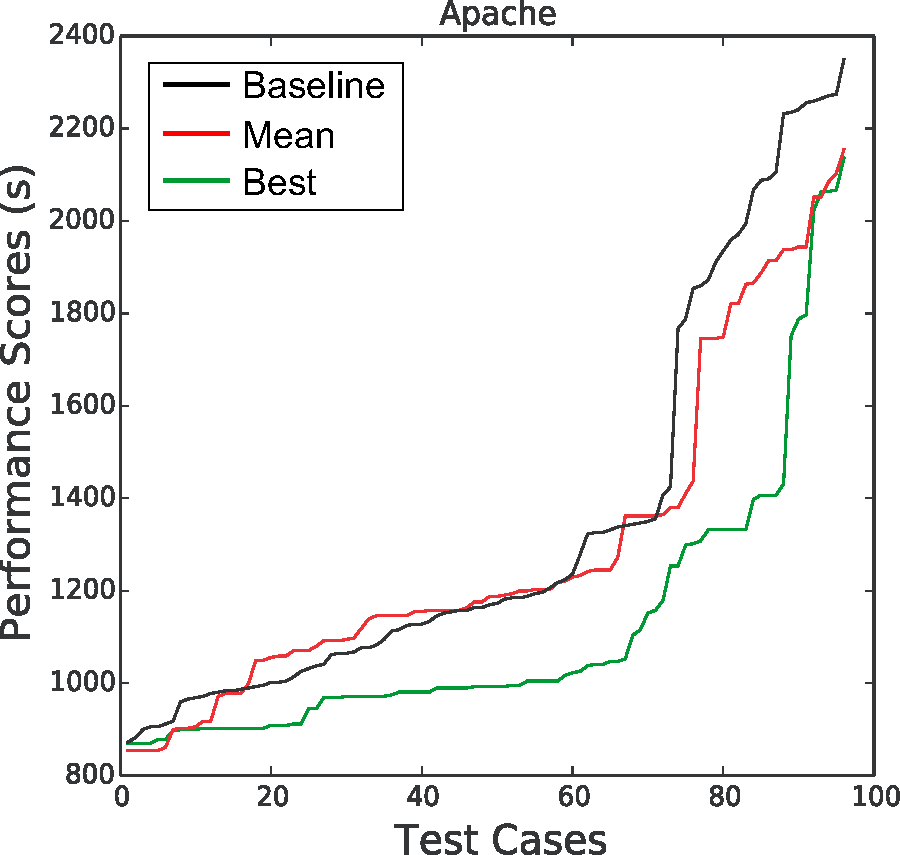
\includegraphics[width=\linewidth]{figs/Apache.pdf}
%\end{minipage}
%\begin{minipage}{0.30\linewidth}
%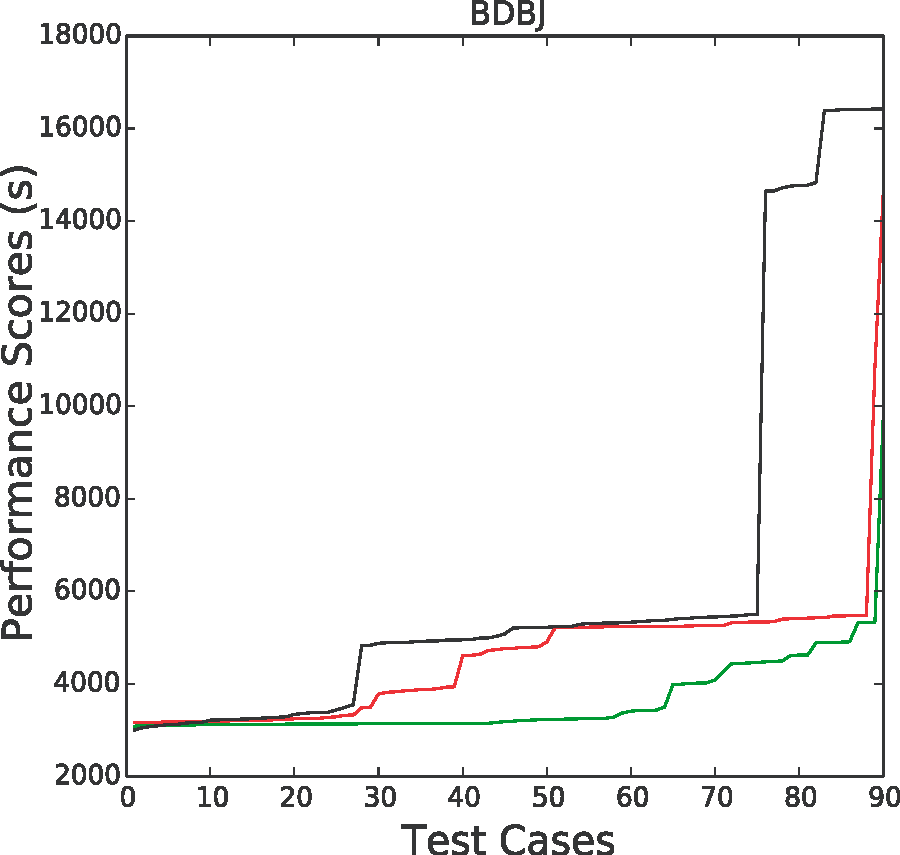
\includegraphics[width=\linewidth]{figs/BDBJ.pdf}
%\end{minipage}
%\begin{minipage}{0.30\linewidth}
%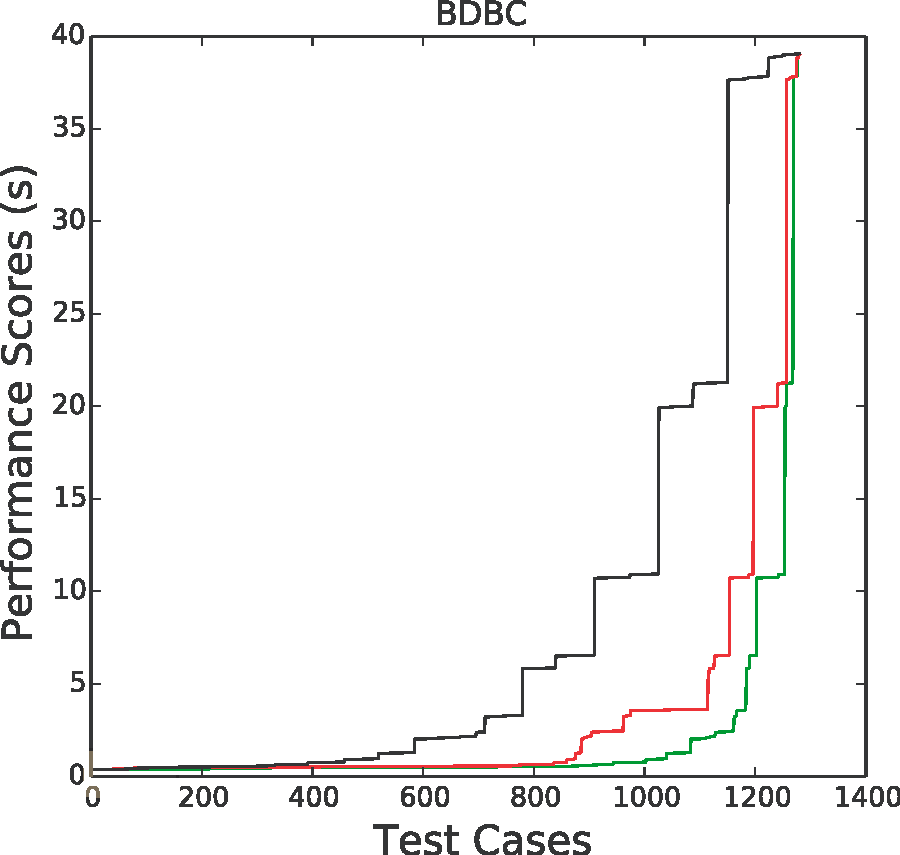
\includegraphics[width=\linewidth]{figs/BDBC.pdf}
%\end{minipage}\\[0.25cm]
%
%\begin{minipage}{0.30\linewidth}
%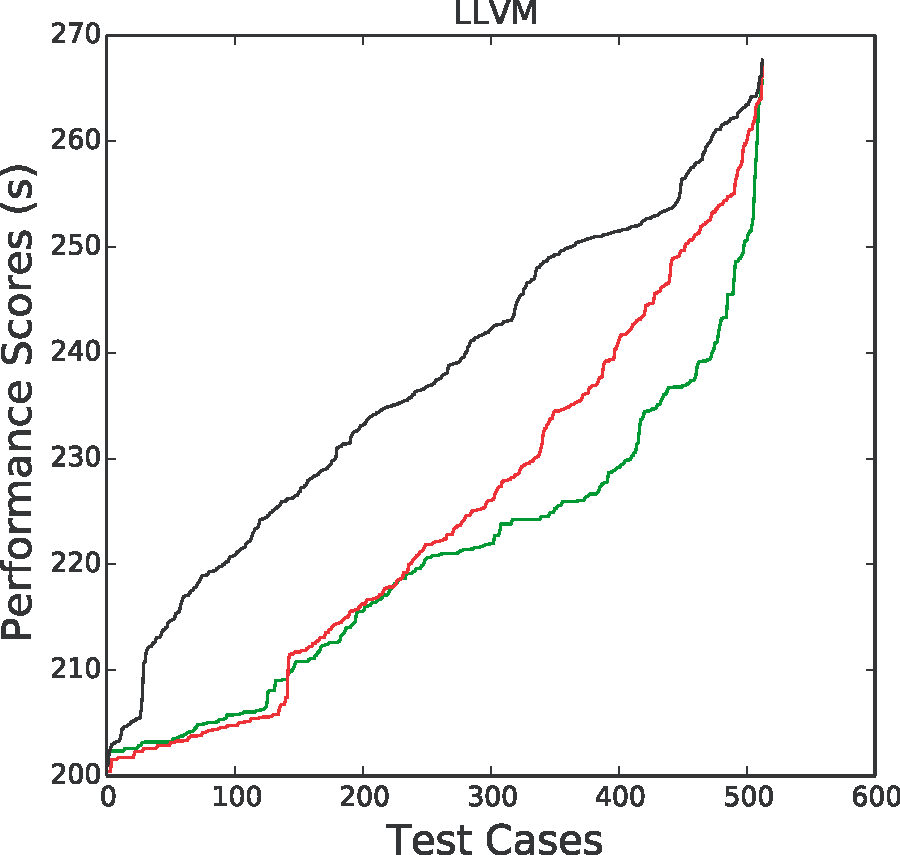
\includegraphics[width=\linewidth]{figs/LLVM.pdf}
%\end{minipage}
%\begin{minipage}{0.30\linewidth}
%includegraphics[width=\linewidth]{figs/SQL.pdf}
%\end{minipage}
%\begin{minipage}{0.30\linewidth}
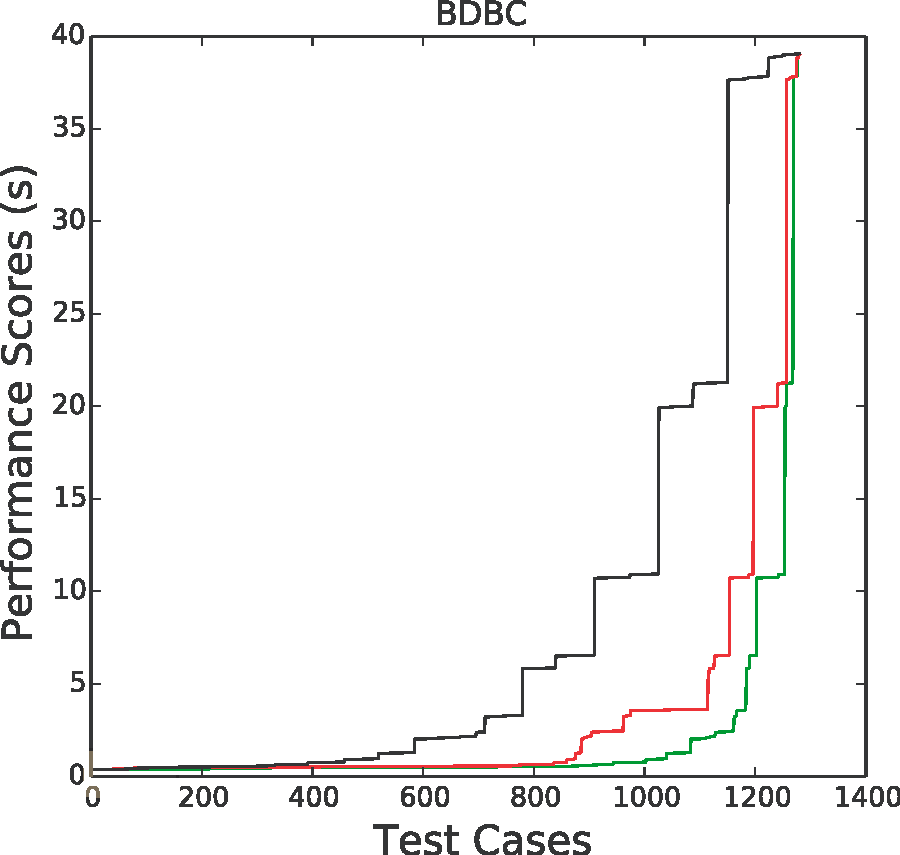
\includegraphics[width=2.5inches]{figs/BDBC.pdf}
%\end{minipage}
\caption{Effects of selecting different kinds of exemplars:
the   \textcolor{black}{\bf  baseline} curve; the
\textcolor{red}{\bf    ``mean''}; and the  
\textcolor{green}{\bf    ``best''} curve.}\label{fig:pp}
\end{figure}



\begin{figure*}[!t]
\scriptsize
   \begin{center}
   \begin{minipage}{.46\linewidth}
    \begin{tabular}{r@{~}|l@{~}|r@{~}|l@{~}|r@{~}|r@{~}|} \cline{2-6}
   & \multicolumn{5}{c|}{ }\\ 
   
   & \multicolumn{5}{c|}{ Data set  properties}\\ 
   & \multicolumn{5}{c|}{  }\\ 
           & \multicolumn{2}{c|}{training}   & \multicolumn{3}{c|}{testing}      \\ \cline{2-6}
   data set      & versions           & cases & versions     & cases    & \% defective             \\ \hline
        jedit    & 3.2, 4.0, 4.1, 4.2 & 1257      & 4.3          & 492          & 2 \\
        ivy      & 1.1, 1.4           & 352       & 2.0          & 352          & 11 \\
        camel    & 1.0, 1.2, 1.4      & 1819      & 1.6          & 965          & 19 \\
        ant      & 1.3, 1.4, 1.5, 1.6 & 947       & 1.7          & 745          & 22 \\
        synapse  & 1.0, 1.1           & 379       & 1.2          & 256          & 34 \\
        velocity & 1.4, 1.5           & 410       & 1.6          & 229          & 34 \\
        lucene   & 2.0, 2.2           & 442       & 2.4          & 340          & 59 \\
        poi      & 1.5, 2, 2.5        & 936       & 3.0          & 442          & 64 \\
        xerces   & 1.0, 1.2, 1.3      & 1055      & 1.4          & 588          & 74  \\ 
        log4j    & 1.0, 1.1           & 244       & 1.2          & 205          & 92   \\
        xalan    & 2.4, 2.5, 2.6      & 2411      & 2.7          & 909          & 99  \\\hline 
        
        
    \end{tabular}\end{minipage}\begin{minipage}{.4\linewidth}
    \begin{tabular}{|rrr|rrr|rr|l} \cline{1-8}
      \multicolumn{8}{|c|}{  }\\
      \multicolumn{8}{|c|}{  Results from learning}\\
       \multicolumn{8}{|c|}{   }\\
   \multicolumn{3}{|c|}{untuned} & \multicolumn{3}{c|}{tuned} & \multicolumn{2}{c|}{change}\\
  \cline{1-8}
  
  pd & pf & good? & pd & pf & good? & pd & pf\\\cline{1-8}
  50 & 27 &   & 64 & 28 & y & 14 & 1&$\star$\\
  65 & 35 & y & 65 & 25 & y & 0 & -10&$\star$\\
  50 & 30 &   & 62 & 41 &   & 12 & 11\\
  66 & 21 & y & 63 & 18 & y & -3 & -3\\
  45 & 18 &   & 47 & 15 &   & 2 & -3\\
  79 & 61 &   & 77 & 61 &   & -2 & 0\\
  55 & 25 &   & 60 & 27 & y & 5 & 2\\
  51 & 32 &   & 61 & 12 & y & 10 & -20&$\star$\\
 30 & 28 &   & 39 & 33 &   & 9 & 5&$\times$\\
  32 & 6 &   & 30 & 9 &   & -2 & 3&$\times$\\
  41 & 5 &   & 48 & 0 &   & 7 & -5&$\times$\\
\hline 
\end{tabular}

\end{minipage}
\end{center}    
  
    \caption{Training and test {\em data set properties} for the Jureczko data sets,
    sorted in ascending order of \% defective examples.
    On the right-hand-side, we show the {\em results from learning}.
    Data is ``good'' if it has   recalls over 60\% and false alarms under 40\%
(and note that, after tuning, there are more ``good'' than before).
Data   marked with ``$\star$'' show large improvements in performance, after tuning.
Data   marked with ``$\times$'' are not ``good'' since their test suites  have so few non-defective examples (less than 5\% of the total sample) that it becomes harder to find better data towards which we can displace test data.
}\label{fig:j}
\end{figure*}




\subsection{Assessment}\label{sect:assess}
In the experiments shown below,  HOW comments  on how to reduce
software defects by adjusting certain static code parameters of the code\footnote{Such parameters can be manually adjusted by programmers or (for large scale changes) automatically adjusted using code refactoring
tools, as shown by Binkely et al. in 2006~\cite{Binkley2006} and more recently by Mkaouer et al. in 2015~\cite{Mkaouer15}.}. How are we to verify that HOW's recommendations actually work? 


As shown in \fig{work}, our proposal divides
project data  into two disjoint sets {\em train} and {\em test}
(so \mbox{{\em train} $\cap ${\em test} $=\;\emptyset$}).
Next, from the train set, we build both a {\em planner} as well
as a {  predictor}. Our general framework does not   commit to any particular  choice
of { planner} or { predictor} but, for the purposes of this paper, 
our { planner}
will be HOW  and our
our { predictors} will be the Random Forest~\cite{Breiman2001} and Random Forest
Regressor taken from the SciKit
Learn toolkit~\cite{Pedregosa2012}.  
%\begin{figure}[t!]
%\small
%\begin{tabular}{|p{.95\linewidth}|}\hline
% Decision tree learners find the attribute whose value's
%select for for sections of the data with least variation in the class
%variable. Decision tree learners then recurse on each selection~\cite{breiman84}. 
%
%A random forest is a set of decision trees, each built
%from some random subset of the rows and columns. The conclusions
%of the forest are a ``vote'' generated by all the trees~\cite{Breiman2001}. 
%
%A standard Random Forest predicts for a discrete class variable while
%a Random Forest Regressor generates numeric predictions.\\\hline
%\end{tabular}
%\caption{Random Forests and Random Forest Regressors.}\label{fig:rr}
%\end{figure}


Turning now to the {\em test} data, this is passed to the { predictor}
to generate a baseline {\em before}  score.
If our { predictors} fail to perform adequately on the test data,
then we cannot trust them to comment on our plans. Accordingly,
if that performance is unsatisfactory, we abort.
Else, we (1)~apply the { planner} to alter the {\em test} data;
then (2)~apply the { predictor} to the altered data {\em test'};
then (3)~return data on the {\em before,after} predictions.



\subsection{When Not to Plan: the Problem of Poor Predictors}\label{sec:notplan}

The clear advantage of the approach of \fig{work} is that it can be readily and automatically
applied to domains with historical data. That said, the obvious drawback with this approach
is that our assessment of the plans is only as good as the predictor. To 
mitigate for this {\em problem of poor predictors}, it is hence wise to demand certain standards for the {\em
satisfactory} threshold used in this \fig{work}. 
 

For example, this study's data from two types of domains: the Jureczko   object-oriented data  
and the Seigmund configuration data. 
For the Seigmund data, the plans generated by HOW advise on how  to change the   configurations settings within a Makefile
(in order to make resulting compiled
code  run faster). Here, performance can be measured in terms of  difference
between the predicted runtime $p$ of test case items and their actual runtimes $a$
using  $s= 100*(1- \frac{abs(a - p)}{a})$.
This paper  explores    six Seigmund configuration data sets:  Berkeley DB (Java and Windows versions), Apache, SQLite, LLVM, and
  x264\footnote{Available from the performance prediction section of PROMISE
  http://openscience.us/repo/performance-predict.}. 
  After splitting that data into equal sized train:test groups, a Random Forest
  Regressor trained on one half, then applied to the other, achieved nearly perfect scores of
%issue 24
\[s=\{99.9, 99.8, 99.4, 99.1, 96,1\}\]
That is, we can be very confident that the predictors from the Seigmund data can assess
HOW's plans.
(Aside: if the reader doubts that such high scores are achievable, we note that these scores are 
consistent with those achieved by predictors built by Seigmund et al.~\cite{sven12}.)


\begin{figure*}[htbp!]
  \renewcommand{\baselinestretch}{0.8}\begin{center}
    {\scriptsize
      \begin{tabular}{c|l|p{4.7in}}
        amc & average method complexity & e.g. number of JAVA byte codes\\\hline
        avg\, cc & average McCabe & average McCabe's cyclomatic complexity seen
        in class\\\hline
        ca & afferent couplings & how many other classes use the specific
        class. \\\hline
class. \\\hline
        cam & cohesion amongst classes & summation of number of different
        types of method parameters in every method divided by a multiplication
        of number of different method parameter types in whole class and
        number of methods. \\\hline
        cbm &coupling between methods &  total number of new/redefined methods
        to which all the inherited methods are coupled\\\hline
        cbo & coupling between objects & increased when the methods of one
        class access services of another.\\\hline
        ce & efferent couplings & how many other classes is used by the
        specific class. \\\hline
        dam & data access & ratio of the number of private (protected)
        attributes to the total number of attributes\\\hline
        dit & depth of inheritance tree &\\\hline
        ic & inheritance coupling &  number of parent classes to which a given
        class is coupled (includes counts of methods and variables inherited)
        \\\hline
        lcom & lack of cohesion in methods &number of pairs of methods that do
        not share a reference to an case variable.\\\hline
        locm3 & another lack of cohesion measure & if $m,a$ are  the number of
        $methods,attributes$
        in a class number and $\mu(a)$  is the number of methods accessing an
        attribute, 
        then
        $lcom3=((\frac{1}{a} \sum, j^a \mu(a, j)) - m)/ (1-m)$.
        \\\hline
        loc & lines of code &\\\hline
        max\, cc & maximum McCabe & maximum McCabe's cyclomatic complexity seen
        in class\\\hline
        mfa & functional abstraction & number of methods inherited by a class
        plus number of methods accessible by member methods of the
        class\\\hline
        moa &  aggregation &  count of the number of data declarations (class
        fields) whose types are user defined classes\\\hline
        noc &  number of children &\\\hline
        npm & number of public methods & \\\hline
        rfc & response for a class &number of  methods invoked in response to
        a message to the object.\\\hline
        wmc & weighted methods per class &\\\hline
        \rowcolor{lightgray}
        defect & defect & Boolean: where defects found in post-release bug-tracking systems.
      \end{tabular}
    }
  \end{center}
  \caption{OO measures used in our defect data sets.  Last line is
    the dependent attribute (whether a defect is reported to  a
    post-release bug-tracking system).}\label{fig:ck}
\end{figure*}

Turning now to the Jureczko   OO data sets, we found:
\bi
\item
Most   predictors in this domain were far from      perfect;
\item 
But several of these predictors could
be salvaged using some sampling and optimization methods (see the notes on SMOTE and differential evolution, below).
\ei
As shown in \fig{j}, we   explore numerous examples of the Jureczko   object-oriented static code data sets: Ant, Camel, Ivy, Jedit,   Log4, Lucene, Poi, Synapse, Velocity, Xalan, Xerces\footnote{Available from the object-oriented defects section of the PROMISE respository openscience.us/repo/defect/ck.}. 
Given access to $V$ released
versions, we test on version $V$ and train on the available data from earlier releases (as
shown in \fig{j}, this means that we are training on hundreds to thousands
of classes and testing on smaller test suites).
Note the three bottom rows marked with $\times$: these contain predominately
defective classes (two-thirds, or more) and in such data sets, it is hard to distinguish
good from bad (since there are so many bad examples). 

For the  Jureczko   data,
the plans generated by HOW advise   how to change static code attributes in order to reduce defects in
Java classes.  Here,
performance can be measured using:
\bi
\item Probability of detection (a.k.a. ``pd'' or recall):  the percent of faulty classes in
the test data detected
by the {\em predictor}.
\item Probability of false alarm (a.k.a. ``pf''): the percent of non-fault
classes that are {\e, predicted} to be defective.
\ei 
The ``untuned'' columns of \fig{j} shows RandomForest's learned {\em pd,pf}
values generated after learning from the training data, then being applied to the test data.
If we define ``good'' to mean $\mathit{pd}>60 \wedge \mathit{pf} < 40$\%,
then only two of our data sets ({\em ivy,ant}) are ``good'' enough. 

The ``tuned'' columns of \fig{j} show that we can salvage some of the data sets.
 Pelayo and Dick~\cite{pelayo07} report that defect prediction is improved by SMOTE~\cite{Chawla2002}; i.e. an over-sampling of minority-class examples.
 Also, Fu et al.~\cite{fu:ase15} report that parameter tuning with differential evolution~\cite{storn97}
can quickly explore the tuning
options of Random Forest to find better settings for the (e.g.) size of the forest, the termination criteria
for tree generation, etc.
The rows marked with $\star$ in \fig{j} show data sets whose performance was improved remarkably by these
techniques. For example, in {\em poi}, the recall increased by 10\% while the false alarm rate dropped by 20\%.
However,  as might have been  expected
we could not salvage the data sets in the  three bottom rows.

In summary, while we cannot trust predictors from some of our defect data sets,
we can plan ways to reduce defects in {\em jedit, ivy, ant, lucene} and {\em poi}.
One important detail to be stressed here is that, when we applied    SMOTE-ing and
parameter tunings, those techniques should be applied the training data and {\em not}
the test data;  
i.e.
we took care that no clues from the test set were ever used in this tuning process.


 

\section{Experiments}

\subsection{Data}
We applied HOW's plans to all  Seigmund data, and the five ``good''
  Jureczko   data sets {\em jedit, ivy, ant, lucene} and {\em poi}.
  The training and tests used for Jurecko were display in \fig{j}. For these data
  sets, training was managed by a Random Forest (tuned in the SMOTED training data using differential
  evolution). \fig{ck} shows Jureczko data attributes.
  
   \fig{cpm} shows the  Seigmund data attributes.
   There were more diverse than the 
    Jurecko data since they
   contain the results of applying many  mutators
  to the configuration options of the Makefiles of  BerkeleyDB (the Java  and  Windows  versions),  Apache,  SQLite,  LLVM, and x264.  


 

\begin{figure}[!t]
\scriptsize
\begin{tabular}{llllll}
  \hline
  \rowcolor{lightgray}
Project & Domain & Lang. & LOC & Features & Config\\\hline
Berkeley DB CE & Database & C & 219,811 & 18 & 2560\\
Berkeley DB JE & Database & Java & 42,596 & 32  & 400\\
Apache & Web Server & C & 230,277 & 9 & 192\\
SQLite & Database & C & 312,625 & 39 & 3,932,160\\
LLVM & Compiler & C++ & 47,549 & 11 & 1024\\
x264 & Video Enc. & C& 45,743 & 16 & 1152\\\hline
\end{tabular}
 
\caption{Seigmund data sets: details on the data sets.
For SQLite, the data  contains 4,553 configurations for prediction modeling and 100 additional random configurations for prediction evaluation, see \cite{vapp}.}\label{fig:cpm}
\end{figure}





   \subsection{Procedures}
  \fig{work} showed how to   build and test HOW's plans.
The    Seigmund and Jureczko data sets have continuous and discrete classes (respectively).
Hence, when building a predictor, we used (1)~Random Forest Regressors for the Seigmund data and (2)~Random Forests
for the Jureczko data.

   For both the Siegmind and Jureczko, we designed a procedure such we had at least
   20 samples from the \fig{work} procedure for  each data set (the value of 20 was choosen as the minimum use sample size via the central limit theorem):
   \bi
   \item
  For the Siegmind data, 
  25 times, 
  we randomized the order of the data, trained on one half (via
  Random Forest Regressor), then tested on the other.
  \item
  For the Jureczko, if we just  used the training and test sets of  \fig{j}, that would only
  give us sample per data set. Such a singleton sample could hide important details since the methods
  used for parameter tuning (SMOTE and differential evolution) use some stochastic sub-routines.
  Hence, for each  of the training sets of \fig{j}, we ran SMOTE+differential evolution 25 times to learn
  parameters for Random Forests.
  \ei
\fig{where} defined two control parameters for HOW:
\bi
\item  $F$   controls the size of the displacement;
\item   $B$   controls how many  attributes are displaced.
\ei
The   25 repeats defined above were executed for various values of $F,B$.
A Scott-Knott procedure was used to test for statistically significant differences in the results.
The Scott-Knott
procedure recommended by Mittas \& Angelis in their 2013
IEEE TSE paper~\cite{mittas13}.  This method
sorts a list of $l$ treatments with $ls$ measurements by their median
score. It then
splits $l$ into sub-lists $m,n$ in order to maximize the expected value of
 differences  in the observed performances
before and after divisions. E.g. for lists $l,m,n$ of size $ls,ms,ns$ where $l=m\cup n$:
 $E(\Delta)=\frac{ms}{ls}abs(m.\mu - l.\mu)^2 + \frac{ns}{ls}abs(n.\mu - l.\mu)^2$.
Scott-Knott  applies an  hypothesis test $H$ to check
if $m,n$ are significantly different. If so, Scott-Knott  recurses on the splits.
 
 

%\begin{figure}[tbp!]
% \subfloat[\label{oracle}]{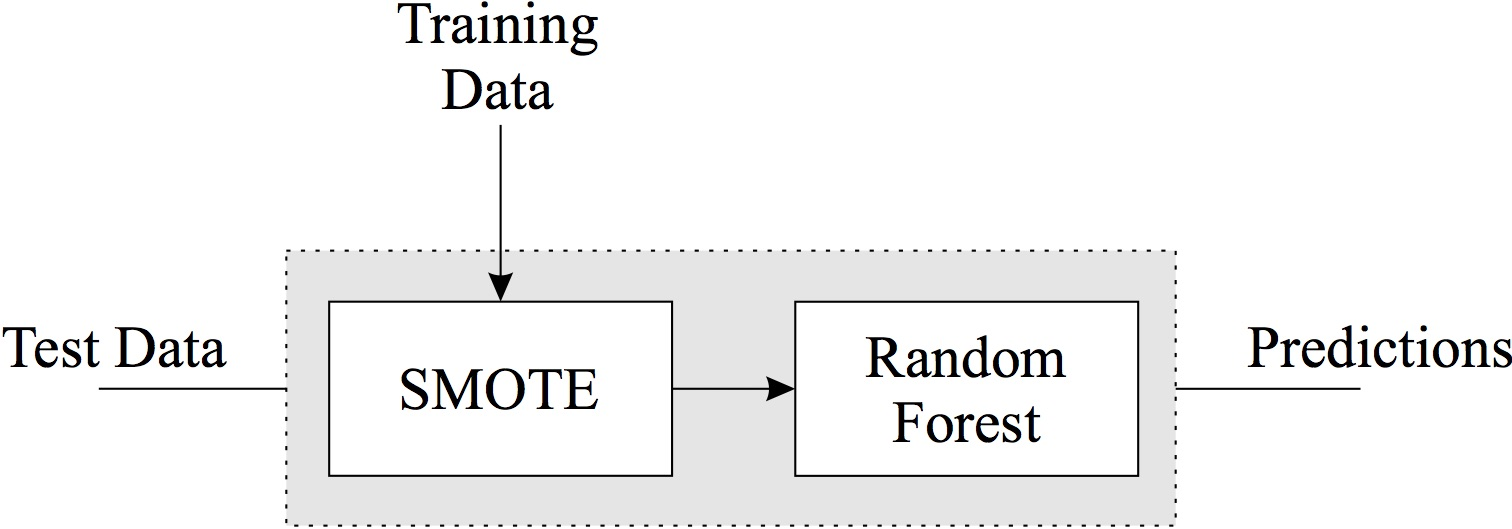
\includegraphics[width=\linewidth]{{figs//Oracle}}\\
%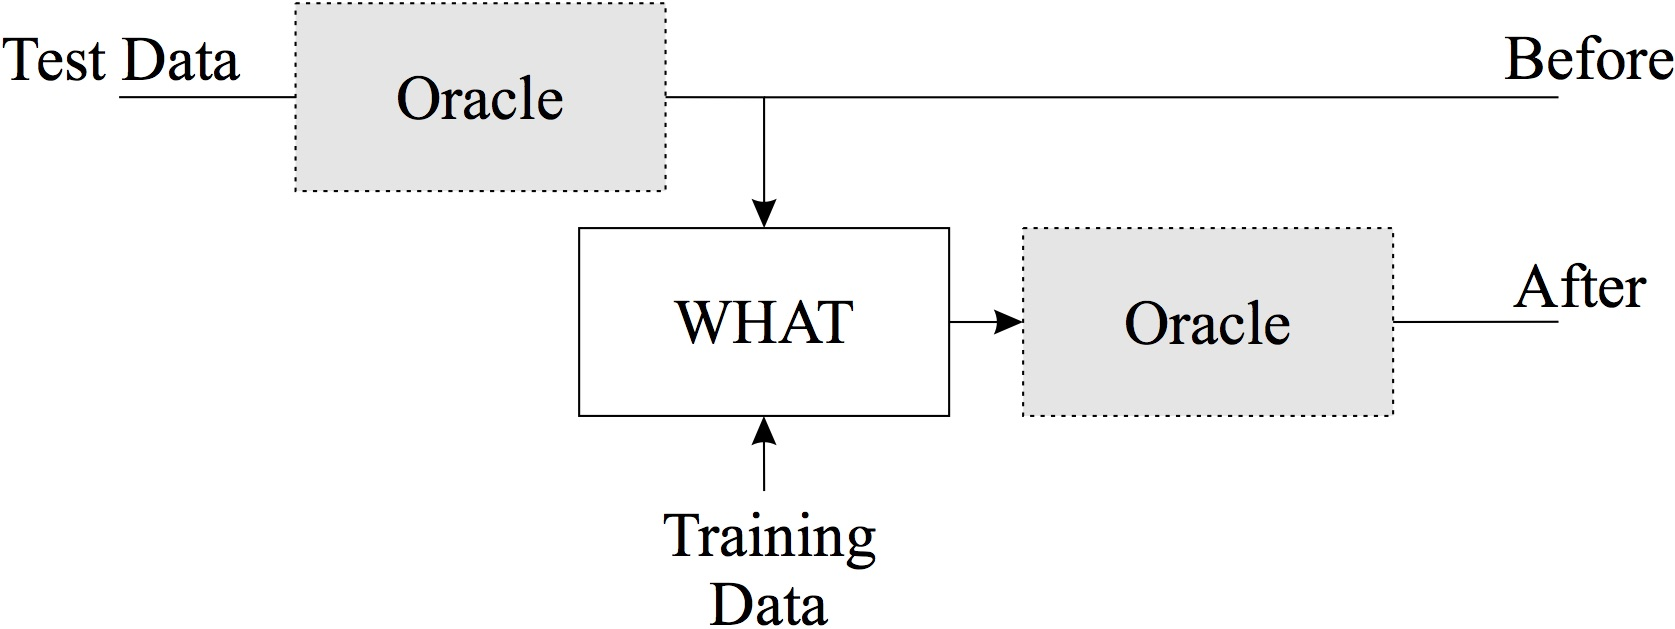
\includegraphics[width=\linewidth]{figs/WHAT}
%\caption{Experimental Rig}
%\label{fig:rig}
  
  
%   \subfloat[Experimental Rig for Defect Prediction]{  \includegraphics[width=\linewidth]{figs/HERE}
%   \label{fig:rig2}}

%\end{figure}

%involves two key components. Firstly, there is the oracle (Random Forest with SMOTE) which is used to make predictions. Then we have the 


%\begin{figure}[tbp]
%\centering
%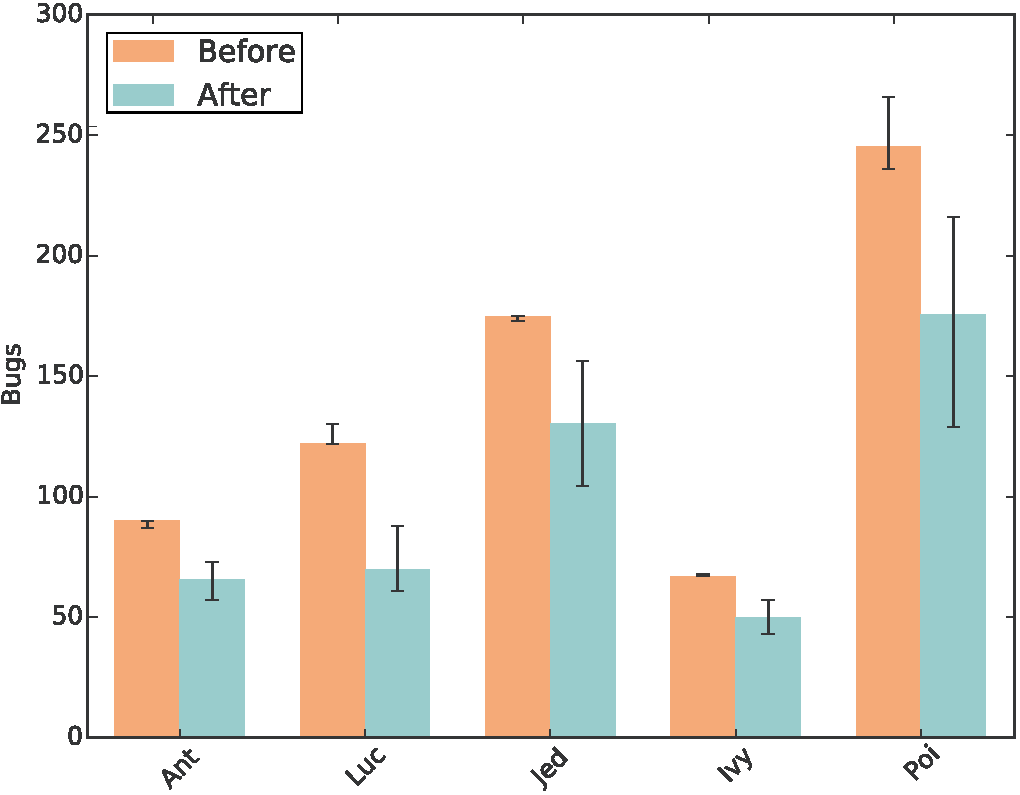
\includegraphics[width=\linewidth]{figs/histograms.pdf}
%\caption{Jureczko object-oriented defect data sets. 
%Comparisons of predictions of defects in the Jureczko data sets before and after planning.}
%\label{fig:bugs}
%\end{figure}

%\subsection{Visualisations of Changes}%

%In this section, we show some sample results. In the next section, we conduct a statistical
%analysis of all   results.

%\fig{bugs} shows the effects of planning on the five good Jureczko data sets. Note that:
%\bi
%\item
%The number of defects predicted in the ``after'' set is always less than ``before'';
%\item
%The reduction can be quite large: e.g. see the over 50\% reduction in the {\em ant} data set.
%\ei
%
%\fig{pp} shows the effects of planning on the Seigmund data sets. The black, red %XXX
%curves show the
%runtimes as predicted in the test sets before/after our planning.  While some of the differences
%are small (eg. LLVM and SQL), some of the others are very large indeed (e.g. the Apache and   BD*).
 
%This visual samples of HOW's planning results look promising-- but they need to be confirmed by a
% more rigorous statistical analysis.
 
\begin{figure*}[!t]
\begin{center}
\begin{minipage}{.44\linewidth}
%\noindent\begin{minipage}{0.5\textwidth}
  {\scriptsize \textbf{Apache}\\[0.1cm]}
  {\scriptsize  \begin{tabular}{{llrrc}}
      \arrayrulecolor{darkgray}
      \rowcolor[gray]{.9} \textbf{Rank} & \textbf{Treatment} & \textbf{Median} & \textbf{IQR} & \\
  1 & F=0.75, B=25 &    0.79  &  0.06 & \quart{0}{11}{7}{49} \\
\hline  2 & F=0.75, B=50 &    0.82  &  0.07 & \quart{7}{14}{13}{49} \\
\hline  3 &  F=0.75, B=100  &    0.85  &  0.06 & \quart{11}{12}{19}{49} \\
  3 & F=0.5, B=25 &    0.87  &  0.03 & \quart{19}{6}{23}{49} \\
  3 & F=0.5, B=50 &    0.87  &  0.07 & \quart{17}{14}{23}{49} \\
\hline  4 &   F=0.5, B=100  &    0.91  &  0.07 & \quart{21}{14}{31}{49} \\
\hline  5 & F=0.25, B=25 &    0.92  &  0.05 & \quart{29}{10}{33}{49} \\
  5 & F=0.25, B=50 &    0.94  &  0.04 & \quart{35}{8}{37}{49} \\
  5 &  F=0.25,B=100   &    0.95  &  0.04 & \quart{35}{8}{39}{49} \\
\hline  6 &     Baseline &    1.0  &  0.0 & \quart{49}{0}{49}{49} \\
\hline \end{tabular}}

\vspace{2mm}\noindent {\scriptsize \textbf{BDBC}\\[0.1cm]}
{\scriptsize  \begin{tabular}{{llrrc}}
\arrayrulecolor{darkgray}
\rowcolor[gray]{.9} \textbf{Rank} & \textbf{Treatment} & \textbf{Median} & \textbf{IQR} & \\
  1 & F=0.75, B=50 &    0.2  &  0.03 & \quart{0}{1}{1}{49} \\
  1 & F=0.75, B=25 &    0.2  &  0.05 & \quart{0}{3}{1}{49} \\
\hline  2 &  F=0.75, B=100  &    0.22  &  0.07 & \quart{1}{5}{2}{49} \\
\hline  3 & F=0.5, B=25 &    0.39  &  0.06 & \quart{11}{4}{12}{49} \\
  3 & F=0.5, B=50 &    0.4  &  0.05 & \quart{12}{3}{13}{49} \\
\hline  4 &   F=0.5,B=100   &    0.45  &  0.08 & \quart{14}{4}{16}{49} \\
\hline  5 & F=0.25, B=25 &    0.65  &  0.05 & \quart{27}{3}{28}{49} \\
  5 & F=0.25, B=50 &    0.66  &  0.05 & \quart{27}{3}{29}{49} \\
\hline  6 &  F=0.25,B=100   &    0.69  &  0.05 & \quart{29}{3}{31}{49} \\
\hline  7 &     Baseline &    1.0  &  0.0 & \quart{49}{0}{49}{49} \\
\hline \end{tabular}}
%\end{minipage}

\vspace{2mm}\noindent{\scriptsize \textbf{BDBJ}\\[0.1cm]}
{\scriptsize  \begin{tabular}{{llrrc}}
\arrayrulecolor{darkgray}
\rowcolor[gray]{.9} \textbf{Rank} & \textbf{Treatment} & \textbf{Median} & \textbf{IQR} & \\
  1 & F=0.75, B=25 &    0.64  &  0.1 & \quart{1}{12}{6}{49} \\
  1 & F=0.75, B=50 &    0.68  &  0.14 & \quart{0}{17}{10}{49} \\
\hline  2 &  F=0.75, B=100   &    0.74  &  0.1 & \quart{12}{12}{18}{49} \\
  2 & F=0.5, B=25 &    0.76  &  0.09 & \quart{15}{11}{20}{49} \\
  2 & F=0.5, B=50 &    0.78  &  0.17 & \quart{15}{21}{23}{49} \\
  2 &   F=0.5,B=100   &    0.8  &  0.07 & \quart{20}{9}{25}{49} \\
\hline  3 & F=0.25, B=25 &    0.85  &  0.05 & \quart{30}{6}{31}{49} \\
\hline  4 & F=0.25, B=50 &    0.89  &  0.09 & \quart{30}{11}{36}{49} \\
  4 &  F=0.25, B=100  &    0.9  &  0.06 & \quart{35}{7}{37}{49} \\
\hline  5 &     Baseline &    1.0  &  0.0 & \quart{49}{0}{49}{49} \\
\hline \end{tabular}}
%\end{minipage}
%\noindent\begin{minipage}{0.5\textwidth}
%  \flushleft
\end{minipage}~~~~~\begin{minipage}{.44\linewidth}
\noindent
{\scriptsize \textbf{LLVM}\\[0.1cm]}
  {\scriptsize  \begin{tabular}{{llrrc}}
\arrayrulecolor{darkgray}
\rowcolor[gray]{.9} \textbf{Rank} & \textbf{Treatment} & \textbf{Median} & \textbf{IQR} & \\
  1 & F=0.75, B=25 &    0.92  &  0.02 & \quart{0}{11}{5}{49} \\
  1 & F=0.75, B=50 &    0.93  &  0.02 & \quart{5}{11}{11}{49} \\
  1 &  F=0.75, B=100   &    0.93  &  0.02 & \quart{11}{11}{11}{49} \\
\hline  2 & F=0.5, B=25 &    0.95  &  0.01 & \quart{16}{6}{22}{49} \\
  2 & F=0.5, B=50 &    0.95  &  0.01 & \quart{16}{6}{22}{49} \\
  2 &   F=0.5, B=100   &    0.96  &  0.01 & \quart{22}{5}{27}{49} \\
\hline  3 & F=0.25, B=25 &    0.97  &  0.01 & \quart{33}{5}{33}{49} \\
  3 & F=0.25, B=50 &    0.98  &  0.0 & \quart{38}{0}{38}{49} \\
  3 &  F=0.25, B=100  &    0.98  &  0.01 & \quart{38}{6}{38}{49} \\
\hline  4 &     Baseline &    1.0  &  0.0 & \quart{49}{0}{49}{49} \\
\hline \end{tabular}}
%\end{minipage}

\vspace{2mm}\noindent {\scriptsize \textbf{SQL}\\[0.1cm]}
  {\scriptsize  \begin{tabular}{{llrrc}}
\arrayrulecolor{darkgray}
\rowcolor[gray]{.9} \textbf{Rank} & \textbf{Treatment} & \textbf{Median} & \textbf{IQR} & \\
  1 & F=0.75, B=25 &    0.98  &  0.0 & \quart{0}{0}{0}{49} \\
  1 & F=0.75, B=50 &    0.98  &  0.0 & \quart{0}{0}{0}{49} \\
  1 & F=0.75, B=100 &   0.99  &  0.01 & \quart{0}{24}{24}{49} \\
  1 & F=0.5, B=25 &    0.99  &  0.0 & \quart{24}{0}{24}{49} \\
  1 & F=0.5, B=50 &    0.99  &  0.0 & \quart{24}{0}{24}{49} \\
  1 & F=0.5, B=100 &    0.99  &  0.01 & \quart{24}{25}{24}{49} \\
  1 & F=0.25, B=50 &    1.0  &  0.0 & \quart{49}{0}{49}{49} \\
  1 & F=0.25-weight-B=25 &    1.0  &  0.0 & \quart{49}{0}{49}{49} \\
  1 & F=0.25, B=100 &    1.0  &  0.0 & \quart{49}{0}{49}{49} \\
  1 &     Baseline &    1.0  &  0.0 & \quart{49}{0}{49}{49} \\
  \hline \end{tabular}}
%\end{minipage}
%\noindent\begin{minipage}{0.5\textwidth}
%  \flushleft

\vspace{2mm}\noindent {\scriptsize \textbf{X264}\\[0.1cm]}
  {\scriptsize  \begin{tabular}{{llrrc}}
\arrayrulecolor{darkgray}
\rowcolor[gray]{.9} \textbf{Rank} & \textbf{Treatment} & \textbf{Median} & \textbf{IQR} & \\
  1 & F=0.75, B=25 &    0.72  &  0.04 & \quart{0}{6}{3}{49} \\
  1 & F=0.75, B=50 &    0.74  &  0.04 & \quart{3}{6}{6}{49} \\
\hline  2 & F=0.5, B=50 &    0.82  &  0.04 & \quart{16}{7}{19}{49} \\
  2 &  F=0.75, B=100  &    0.82  &  0.06 & \quart{13}{10}{19}{49} \\
  2 & F=0.5, B=25 &    0.82  &  0.03 & \quart{19}{5}{19}{49} \\
\hline  3 &   F=0.5, B=100   &    0.88  &  0.03 & \quart{26}{5}{29}{49} \\
\hline  4 & F=0.25, B=50 &    0.91  &  0.02 & \quart{33}{3}{34}{49} \\
  4 & F=0.25, B=25 &    0.91  &  0.02 & \quart{34}{4}{34}{49} \\
\hline  5 &  F=0.25, B=100 &    0.93  &  0.02 & \quart{36}{3}{38}{49} \\
\hline  6 &     Baseline &    1.0  &  0.0 & \quart{49}{0}{49}{49} \\
\hline \end{tabular}}
\end{minipage}

\end{center}
\caption{Results on  Seigmund   data sets. Baseline values shown at bottom. All other values
are ratios of baselines.
Recall that $B$ denotes how what {\em percent} of the attributes are displaced
and $F$ denotes how {\em far} the test cases are mutated (so at $F=0.75,B=100$, all
attributes are displaced 75\% of the distance to the exemplar).
For each of the  tables in this figure, better methods appear higher up. In these tables, median and IQR are the 50th and the (75-25)th percentiles. The IQR ranges are shown in the right column with black dot at the median. Horizontal lines divide the “ranks” found by Scott-Knott (shown in left column).
}\label{fig:jur}
\end{figure*}


\begin{figure}[!t] 
  {\scriptsize \textbf{Ant}\\[0.1cm]}
  {\scriptsize  \begin{tabular}{{l@{~~~~}l@{}r@{~~~~}r@{~~}c@{}r}}
      \arrayrulecolor{darkgray}
      \rowcolor[gray]{.9} \textbf{Rank} & \textbf{Treatment} & \textbf{Median} & \textbf{IQR} && \textbf{Bugs}\\
   1 &  F=0.75, B=100 &    0.71  &  0.19 & \quart{0}{25}{10}{49} & 62 \\
\hline  2 &   F=0.5, B=100  &    0.88  &  0.14 & \quart{20}{19}{33}{49} & 77\\
\hline  3 & F=0.5, B=50\% &    0.91  &  0.08 & \quart{32}{11}{37}{49} & 80\\
  3 & F=0.75, B=50\% &    0.92  &  0.09 & \quart{31}{12}{39}{49} & 82\\
  3 &  F=0.25, B=100  &    0.92  &  0.04 & \quart{36}{5}{39}{49} & 81\\
  3 & F=0.75, B=25\% &    0.94  &  0.09 & \quart{36}{12}{41}{49} & 82\\
\hline  4 & F=0.25, B=50\% &    0.97  &  0.03 & \quart{44}{4}{45}{49} & 86\\
  4 & F=0.5, B=25\% &    0.98  &  0.06 & \quart{40}{8}{47}{49} & 86\\
\hline  5 &F= 0.25, B=25\% &    0.99  &  0.01 & \quart{48}{1}{48}{49} & 87\\
\hline  6 &         Base &    1.0  &  0.0 & \quart{49}{0}{49}{49} & 90\\
\hline \end{tabular}}
%\end{minipage}\\[0.1cm] 

%\noindent\begin{minipage}{0.5\textwidth}
 % \flushleft
 \vspace{2mm}
 \noindent {\scriptsize \textbf{Ivy}\\[0.1cm]}
{\scriptsize  \begin{tabular}{{l@{~~~~}l@{}r@{~~~~}r@{~~~~}c@{}r}}
\arrayrulecolor{darkgray}
\rowcolor[gray]{.9} \textbf{Rank} & \textbf{Treatment} & \textbf{Median} & \textbf{IQR} & & \textbf{Bugs}\\
  1 &  F=0.75,  B=100 &    0.75  &  0.18 & \quart{0}{29}{8}{49} & 50\\
\hline  2 &   F=0.5,B=100   &    0.84  &  0.08 & \quart{14}{14}{23}{49} & 56\\
  2 & F=0.75, B=50 &    0.84  &  0.09 & \quart{18}{15}{23}{49} & 56\\
\hline  3 & F=0.5, B=50 &    0.91  &  0.05 & \quart{29}{9}{34}{49} & 61\\
\hline  4 & F=0.25, B=50 &    0.96  &  0.01 & \quart{43}{1}{43}{49} & 64\\
  4 & F=0.75, B=25 &    0.96  &  0.05 & \quart{39}{9}{43}{49} & 65\\
  4 &  F=0.25, B=100  &    0.97  &  0.05 & \quart{39}{9}{44}{49} & 65\\
  4 & F=0.5, B=25 &    0.97  &  0.03 & \quart{43}{5}{44}{49} & 65\\
\hline  5 & F=0.25, B=25 &    0.99  &  0.01 & \quart{48}{1}{48}{49} & 66\\
\hline  6 &         Base &    1.0  &  0.0 & \quart{49}{0}{49}{49} & 67\\
\hline \end{tabular}}
%\end{minipage}\\[0.1cm] 

%\noindent\begin{minipage}{0.5\textwidth}
 % \flushleft
\vspace{2mm}\noindent{\scriptsize \textbf{Jedit}\\[0.1cm]}
  {\scriptsize  \begin{tabular}{{l@{~~~~}l@{}r@{~~~~}r@{~~~~}c@{}r}}
\arrayrulecolor{darkgray}
\rowcolor[gray]{.9} \textbf{Rank} & \textbf{Treatment} & \textbf{Median} & \textbf{IQR} & & \textbf{Bugs}\\
  1 &  F=0.75,  &    0.76  &  0.21 & \quart{0}{28}{17}{49} & 130\\
  1 &   0.5,  &    0.76  &  0.16 & \quart{9}{22}{17}{49} & 131\\
\hline  2 & 0.75, B=50\% &    0.85  &  0.12 & \quart{22}{17}{29}{49} & 146\\
\hline  3 &  0.25,  &    0.87  &  0.07 & \quart{28}{9}{32}{49} & 152\\
\hline  4 & 0.5, B=50\% &    0.93  &  0.05 & \quart{37}{7}{40}{49} & 162\\
\hline  5 & 0.25, B=50\% &    0.97  &  0.03 & \quart{43}{4}{45}{49} & 167\\
  5 & 0.75, B=25\% &    0.97  &  0.02 & \quart{44}{3}{45}{49} & 168\\
\hline  6 & 0.5, B=25\% &    0.98  &  0.02 & \quart{45}{3}{47}{49} & 170\\
  6 & 0.25, B=25\% &    0.98  &  0.01 & \quart{47}{1}{47}{49} & 171\\
\hline  7 &         Base &    1.0  &  0.0 & \quart{49}{0}{49}{49} & 175\\
\hline \end{tabular}}
%\end{minipage}\\[0.1cm] 

%\noindent\begin{minipage}{0.5\textwidth}
%  \flushleft
\vspace{2mm}\noindent{\scriptsize \textbf{Lucene}\\[0.1cm]}
  {\scriptsize  \begin{tabular}{{l@{~~~~}l@{}r@{~~~~}r@{~~~~}c@{}r}}
\arrayrulecolor{darkgray}
\rowcolor[gray]{.9} \textbf{Rank} & \textbf{Treatment} & \textbf{Median} & \textbf{IQR} & & \textbf{Bugs}\\
  1 &  0.75,  &    0.66  &  0.2 & \quart{0}{21}{13}{49} & 97\\
\hline  2 & 0.75, B=50\% &    0.7  &  0.1 & \quart{14}{10}{17}{49} & 103\\
\hline  3 & 0.75, B=25\% &    0.8  &  0.09 & \quart{21}{10}{28}{49} & 117\\
  3 &   0.5,  &    0.81  &  0.09 & \quart{26}{9}{29}{49} & 119\\
\hline  4 & 0.5, B=50\% &    0.88  &  0.07 & \quart{34}{8}{36}{49} & 128\\
  4 & 0.25, B=25\% &    0.89  &  0.07 & \quart{36}{8}{38}{49} & 130\\
  4 &  0.25,  &    0.92  &  0.04 & \quart{39}{4}{41}{49} & 133\\
\hline  5 & 0.25, B=50\% &    0.95  &  0.04 & \quart{42}{4}{44}{49} & 139\\
  5 & 0.5, B=25\% &    0.96  &  0.03 & \quart{43}{3}{45}{49} & 141\\
\hline  6 &         Base &    1.0  &  0.0 & \quart{49}{0}{49}{49} & 146\\
\hline \end{tabular}}
%\end{minipage}\\[0.1cm] 

%\noindent\begin{minipage}{0.5\textwidth}
%  \flushleft
\vspace{2mm}\noindent{\scriptsize \textbf{Poi}\\[0.1cm]}
  {\scriptsize  \begin{tabular}{{l@{~~~~}l@{}r@{~~~~}r@{~~~~}c@{}r}}
      \arrayrulecolor{darkgray}
\rowcolor[gray]{.9} \textbf{Rank} & \textbf{Treatment} & \textbf{Median} & \textbf{IQR} & & \textbf{Bugs}\\
  1 &  0.75,  &    0.72  &  0.26 & \quart{0}{29}{18}{49} & 173\\
\hline  2 & 0.75, B=50\% &    0.79  &  0.15 & \quart{14}{17}{26}{49} & 190\\
  2 &   0.5,  &    0.81  &  0.14 & \quart{21}{16}{28}{49} & 195\\
\hline  3 & 0.5, B=50\% &    0.9  &  0.11 & \quart{30}{13}{38}{49} & 217\\
  3 &  0.25,  &    0.91  &  0.05 & \quart{36}{6}{39}{49} & 219\\
\hline  4 & 0.75, B=25\% &    0.94  &  0.05 & \quart{39}{6}{43}{49} & 226\\
  4 & 0.25, B=50\% &    0.94  &  0.06 & \quart{39}{7}{43}{49} & 226\\
\hline  5 & 0.25, B=25\% &    0.96  &  0.03 & \quart{44}{3}{45}{49} & 231\\
  5 & 0.5, B=25\% &    0.96  &  0.03 & \quart{44}{3}{45}{49} & 231\\
\hline  6 &         Base &    1.0  &  0.0 & \quart{49}{0}{49}{49} & 240\\
\hline \end{tabular}}
%\end{minipage}
\caption{Results on  Jureczko   data sets. Same format as \fig{jur}.}
\label{fig:ant}
\end{figure}


For this study, our hypothesis test $H$ was a
conjunction of the A12 effect size test of  a
non-parametric bootstrap sampling; i.e. our
Scott-Knott divided the data if {\em both}
bootstrapping and an effect size test agreed that
the division was statistically significant (99\%
confidence) and not a ``small'' effect ($A12 \ge
0.6$).
For a justification of the use of non-parametric
bootstrapping, see Efron \&
Tibshirani~\cite[p220-223]{efron93}.
For a justification of the use of effect size tests
see Shepperd\&MacDonell~\cite{shepperd12a}; Kampenes~\cite{kampenes07}; and
Kocaguenli et al.~\cite{Kocaguneli2013:ep}. These researchers
warn that even if an
hypothesis test declares two populations to be
``significantly'' different, then that result is
misleading if the ``effect size'' is very small.
Hence, to assess 
the performance differences 
we first must rule out small effects using A12, 
a test   recently 
endorsed by Arcuri and Briand
at ICSE'11~\cite{arcuri11}.
 
  
\subsection{Results}
The results for each data set, for different ranges of $(F,B)$ are shown in \fig{jur} and \fig{ant}.
Also included are a {\em baseline} figure which is taken from the cases in the test data
and  Since we wish to demonstrate
improving defects
(for Jureczko data) and runtimes (for the Seigmund data), all our results are presented as ratios of the baseline (so numbers less than 1.0 indicate improvements).

  
 The   results of \fig{jur} and \fig{ant} show that in $\frac{10}{11}$ of our
 data sets, the baseline results are ranked significantly worse than the results seen
 after planning (evidence: the statistical ranking assigned by Scott-Knott is shown in the left-hand-side columns and most baselines get larger, i.e. worse, ranks
 that the treated data). The exception to this is SQL in  \fig{jur}. which
 seems to
 be resistant to our planning methods.
 
 By comparing the top and bottom line of results from each data set, we can see how much HOW's
 plans effect the predicted values. While the  size of the change varies from data set to data set:
 \bi
 \item The median change is down to 72\% and 75\%  of the original baseline values for Seigmund and Jureczko, respectively;
 \item The best change is down to 20\% and 66\% of the original baseline values for Seigmund and Jureczko, respectively;
 \ei
 As to the impact of changing how far we mutate (the $F$ value) or how many attributes
 we mutate (the $B$ value), the results are different for the data sets with discrete and continuous attributes:
 \bi
 \item For data sets with continuous objectives (the Jureczko data of \fig{jur}),
 best results are obtained by taking the fewest attributes (minimize $B$) 
 while moving close to the exemplar (maximize $F$).
 \item For data sets with discrete objectives (the Seigmund data  of \fig{ant}),
 best results are obtained by maximizing both $F$ and $B$.
 \ei
  From these differences, we conclude that the more specific the  information used for exemplar
 generation, the better the planning. Recall that for the discrete
 attributes, the exemplar is the mean position of all cases in the cluster.
 However,  for continuous
 objectives, the exemplar is much more specific and is the  single  best case in a cluster 

% \section{Discussion}
\section{Threats to validity}

 

As with any empirical study, biases can affect the final results. Therefore, any
conclusions made from this work must be considered with the following issues in
mind.


{\em 1. Evaluation bias:} The biggest threat to validity of this work is our use
of predictors learned on the training data to assess the impact of HOW's plans
on the test data.
If we believe the outputs of those predictors, then we can also believe that
\fig{jur} and \fig{ant} are showing true effects.  

%XXX begin rahul 
One way to assess the validity of our predictions is to consider the space that generates
them. \fig{howxy} is from the {\em ivy} data
set. It shows (1)~the training cases and (2)~the test cases and (3)~the
test cases displaced after applying HOW's plans.
To generate that figure, we placed all of 1+2+3 into the same data set then computed the first
two  components (using PCA). Note that the  the   displaced test
cases  (shown in green)  fall closer to the training cases (shown in gray) than
the test cases (shown in red).  That is, if we believe
that the gray data is  suitable for assessing
the test cases (as indicated by the {\em ivy} results from \fig{j}), then it follows
that we believe even more in the predictions
generated from the displaced data).

This pattern of \fig{howxy} (where the displaced test cases are found closer to  the training cases than the test cases) has been observed in all the other data sets studied in this
paper. Hence,  we can assert that
predictors learned from these training data have some authority in the regions
used to generate the plans\footnote{If the reader is concerned that this 2d projection
losses important information, then they should note that two separate  studies~\cite{papa13,divya15}
have confirmed that building defect predictors from this 2d space are just as effective
as predictors learned using all the defect attributes of \fig{ck}.}. 


\begin{figure}
\begin{center}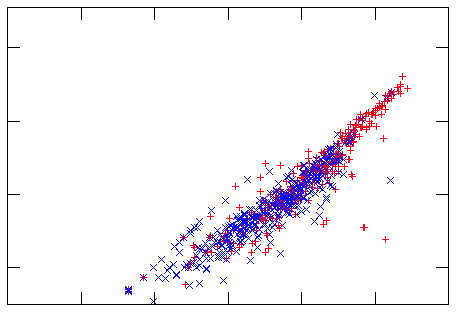
\includegraphics[width=3in]{figs/2d.png}\end{center}
\caption{Training cases (in gray), test cases (in red) and 
test cases displaced by HOW (in green). Note how the green (displaced) cases are closer to the  training
date than the original test data
i.e. predictors trained on the training cases and
applied to the test cases should
work just as well, or better, on the displaced test cases.}\label{fig:howxy}
\end{figure}
%XXX end

That said, one thing to be said here
is that we {\em strongly} recommend that predictors are assessed prior to planning.
We showed above the results of one such planning exercise- we noted that half
our defect data sets are not clear enough to support planning. On the other hand,
the predictors from the configuration domain are extraordinarily accurate (recall
their near perfect predictions seen in \tion{notplan}).

 
{\em 2. Learner bias: } For building the defect predictors in this study, we elected
to use  Random Forest  and Random Forest Regressors .
We chose this approach,  based on its reputation for having the better  performance of 
21 other learners for defect prediction~\cite{lessmann}.
Data mining is a
large and active field and any single study can only use a small
subset of the known classification algorithms.  


{\em 3. Sampling bias} threatens any data mining experiment; i.e., what matters
there may not be true here. For example, the data sets used here comes from two sources
(Seigmund et al. and Jureczko et al.) and any biases in their selection procedures
threaten the validity of these results. 
That said,
the best we can do is define our methods and publicize our data and code so that other researchers can
try to repeat our results and, perhaps, point out a previously unknown bias
in our analysis. Hopefully, other researchers will emulate our methods in
order to repeat, refute, or improve our results. 



%%\footnote{LL: It seems to me that $privacy$ in LACE approach could be compromised in the case of extremes if I had some knowledge of the parties. Consider a case where you know that a bunch of startups and Microsoft contributed to a private cache. Even with the random perturbation in MORPH, it will be REALLY obvious which defect data came from Windows vs. all of the others because Windows will have LOC orders of magnitude greater than anyone else, right?}
 
%XXXX everytime it says LACE, do you mean LACE2

%{\em 4. Comparison bias:}
%There are many privacy algorithms~\cite{Fung2010survey} and it would be difficult to 
%compare their performances (especially with various ways to measure privacy).
%In this work, we use LACE.

%{\em 5. Other Evaluation Bias:}
%The utility of  obfuscated data can be measured
%semantically (where the workload is unknown) or empirically (known workload
%e.g., classification or aggregate query answering). In this work we measure
%utility empirically for defect prediction only.


%

\section{Related Work}

 

HOW is more a data mining method than a model-based optimizer. It represents our next attempt
to develop model-less instance-based optimizers.  Our previous attempts in this area
were the W2, WHERE, and IDEA systems~~\cite{menzies13:brady,Menzies2013:local,me12c}.
W2 was developed with Brady et al.~\cite{menzies13:brady}. 
W2 reasoned over deltas in the the raw
attributes values (and not the synthesized attributes used by HOW). 
The results of  adjusting values via those deltas was assessed via an SQL-like
query that selected all examples in the database that satisfied the newly adjusted
values. W2 suffers from two problems that are resolved
in this paper: {\em optimization failure} and {\em instance exhastion}.
\bi
\item 
As reported in that paper, W2
had a large number of {\em optimization failures}; i.e. after applying its recommendations,
the objective scores actually got worse. We recommend HOW's approach (of reasoning
over the synthesized attributes) to W2 since {\em in none of the above
results} do we observe that {\em after} we treat the data, that the objective scores are worse.
\item
As to {\em instance exhaustion}, W2 was a simple case-based reasoning system that never generalized
over its instances. Hence, the SQl-like query used to asses W2's plans often returned
a vanishingly small number of instances. To avoid this problem, we strongly recommend
combining a planning system with a prediction system (as done in this paper) such that we can
generalize to adjusted examples not seen on the original sample.
\ei
The WHERE tool~\cite{Menzies2013:local} developed the recursive clustering method over synthesized attributes
  used in this paper. WHERE was   a prediction
system since reported current patterns in the data, rather than proposing plans
on how to improve those patterns. Nor did that tool offer guidance on how to assess
the results of stepping along those patterns to guide changes to the system.

The problems of W2 and the success of WHERE suggested in might be useful to combine
WHERE's synthesized attributes with W2. The result was the IDEA tool~\cite{me12c}. 
While the initial prototype seemed promising~\cite{me12c}, we made the mistake of using
the tree structure of the recursive clusters to generate plans (in IDEA, the plan to
move an instance from one poorly performing cluster $C_1$ to another $C_2$ was computed
from the different in the  median
values of the instances in the two  branches that lead to $C_1$ and $C_2$).  When
that approach was applied to the data used in this paper, the results were quite weak
(very little net improvement). However, we abandoned the tree-query approach
and went for the pure instance-based approach discussed at the start of this paper.


Moving on to other releated work, depending on the audience  we would
 call HOW a {\em spectral learner}, 
a {\em response surface method}, or  a {\em local search operator}.
According to
Kamvar et al~\cite{kamvar03}
{\em spectral learners}reason across $m$ underlying dimensions synthesized
using (say) PCA~\cite{pearson1901}. For example,
algorithms like PDDP~\cite{boley98} use PCA to
recursively divide data into smaller regions where each level of recursion needs an   $O(N^2)$ analysis
to infer the principle components. HOW performs an analogous procedure using a   $O(2N)$ analysis
based on a heuristic proposed by
Faloutsos and Lin~\cite{Faloutsos1995} (see above, the ``FASTMAP'' algorithm).

{\em Response surface methods}  build a fast approximation to the function being optimized,
then uses that  approximation to take intelligent guesses about useful mutations. HOW
is a non-parametric response surface method that finds its response surface via recursive
clustering. For an example of a parametric response surface method, that uses Gaussian process
models, see Zuluaga et al.~\cite{zuluaga13}.

A {\em local search operator} that a some probability $p$, nudges  instance variables
along a dimension that improves its objective scores. HOW's recursive clustering methods
combine $n$ dimensions into $m \ll n$ so its ``nudges'' are simultaneous
adjustments along multiple dimensions. For an example of other kinds of local search algorithms, that only adjust
one variable at a time, see the literature on WALKSAT~\cite{Selman1992} and MAXWALKSAT~\cite{kautz97}.
See also the literature on local search methods in multi-objective optimization.
For example,
Peng et al.~\cite{peng09:ls} have augmented MOEAs with
local search  (i.e. applying a problem-specific repair/improvement
heuristic on some current solution).
Also, Igel et al.'s~\cite{igel07} multi-objective
covariance matrix adaptation evolution strategy
can run the mutations along  ``ridges'' in the search space.

Note that the above response surface methods and local search operators cannot be compared to HOW
since, unlike HOW, they assume the presence of some model that can evaluate generations of newly mutated
instances. Recall from the above that the goal of HOW is to offer an optimization method without
using the evolutionary methods that make extensive demands on an underlying domain model.



 
 \subsubsection{Aside: Can We Call These Plans ``Causal''?}
With one additional stipulation,   this framework can be used to check if the learned
plans can be said to {\em cause} a change in the domain being explored.

In the literature, there are two main definitions of causality: Hill's H-causality~\cite{Hill1965}
and Granger's G-casualty~\cite{granger80}. 
An effect
is H-causal if it satisfies nine criteria\footnote{Hill's criteria for
demonstrating causality:
{\em  plausibility};
{\em strength} of the effect;
{\em 
specificity}, i.e. locality of the effect
to specialized groups;
{\em
support} by experimental evidence;
{\em 
coherence} between cause-effects noted
in the field and in laboratory samples;
{\em
temporally} i.e. the effect has to follow the cause;
{\em 
analogy}, i.e.  similar causes have similar effects;
{\em
biological gradient}, i.e.  more exposure to the cause leads to more of an
effect; and
{\em
consistency}, i.e.  the same cause-effect pairings have been seen by different persons
in different places.}
It is hard to demonstrate H-causality in software engineering.
For example, Hill's criteria emphasises repeatability and laboratory studies-- both of which are
hard to perform in software engineering (e.g. see the continued debate about
the value of using undergraduate students to surrogates for industrial
practitioners in software engineering research~\cite{Carver2003}). Also, Hill's requirement
for consistent results is far easier to achieve in studies of small closed systems (e.g. bacteria in a petri dish)
than in large socio-technical systems (e.g. open source projects). In the latter,
effects are more {\em probabilistic} than {\em categorical}-- by which we mean that 
some cause tends to cause some effect at some probability $p$ less that one.
This in turn means that at some probability $q$ (where $0 \le q < p \le 1$)
that we will find examples of {\em inconsistency} where some cause does {\em not} lead
to some effect (thus violating one of Hill's criteria for demonstrating causality).

The  difficulties associated with Hill's criteria lead Granger~\cite{granger80}
to propose another more practical criteria\footnote{Granger  himself comments that
his proposal was based on earlier work by Norbert Weiner~\cite{Seth2007}.}.
\mbox{G-causality} is based on building predictions based on {\em past} data,
then showing that this works for {\em future} data~\cite{granger80}. 
 In  \fig{work}, we demand that the {\em test}
data is not necessarily collected before the {\em train} data:
\bi
\item[\#1:] For data collected from software released in multiple versions, we should hence use  versions  $i,j$ to build models that are applied to version  $k$ where $i<j<k$.
\item[\#2:] For data collected from Monte Carlo simulations (where inputs are selected at random)
then as long as simulation $i$ is not used to adjust simulation $j> i$, then any item in that
data could be generated before any other. For this kind of data, we  can use the first $X\%$
of the simulation for training, and the remaining data for testing.
\ee
In the two case studies of this paper, the Jureczko object-oriented defect data comes from software
released in multiple versions while the Seigmund configuration data comes from Monte Carlo simulations.
Hence, we use procedure \#1 for the defect data and procedure \#2 for the configuration data.

With these changes,
we can reasonably claim that the plan's generating by HOW are G-causal.


\section{Conclusion}
% \section*{Acknowledgements}
 
This paper has explored the problem of assess changes to a project without
extensive field studies. We have proposed using predictors learned from domain data
to serve as the oracle that judges the effectiveness of those changes.

The novel features of this paper are
\be
\item A general framework for using  predictive system to build planners (see \fig{work}).
For this paper, we used Random Forests as our predictor, but other predictors could
serve just as well.
\item A  test to recognizes  when we should {\em not}  plan: specifically,
planning is
not recommended in domains with  poorly performing predictors. In this paper, that
test excluded certain problematic defect data sets.
\item The HOW  case-based planner, which has not been presented before. HOW
is a significant improvement on our two prior implementations~\cite{6600685,me12c} that both
suffered
from {\em optimization failure}; i.e. when their recommendations were applied,
the resulting behavior actually got worse. We recommend HOW over that prior work
since none of our results exhibited such optimization failures.
\item The experiments of this paper, which showed that 
the HOW planner is useful for real-world tasks;
e.g. significantly reducing the
predicted values of the Jureczko software defects and the Seigmund software runtimes.
For those data sets, HOW
reduce
 the predicted values of defect counts and  runtimes to    
 72\%,75\%  (median) and 66\%,20\% (best case) of the initial values.
\ee 
As to when we would {\em not} use HOW, if  a domain has an accessible
and certified and well-maintained
domain model, then we would go beyond CBR and apply algorithms that can take
full advantage of the domain knowledge in those models; e.g. GALE, NSGA-II, NSGA-III, SPEA2, IBEA, particle swarm optimization, MOEA/D, etc.~\cite{krall14,deb00a,zit02,zit04,%
deb14,Cui2005a,zhang07:TEC}. 

That said, one clear future direction would be explore
combinations of CBR tools with other approaches. 
One way to view HOW is a {\em local patch operator} that could be applied within 
GALE, NSGA*, etc (so in that combination, we would be trying to use   HOW's local patches to 
to optimize those optimizers).
 

\section*{Acknowledgments}

The work has partially funded by a National Science Foundation CISE CCF award \#1506586.
 
\bibliography{how}{}
\bibliographystyle{IEEEtran}
\balance
\end{document}
